%*************************************************************************************************************
% PREAMBLE STUFF
%*************************************************************************************************************
% Instead of inserting my \usepackage and defined commands here, I keep them in a separate file
% Queen's Thesis Format
% (Borrowed from Dean Jin's BigDis.tex file, then heavily modified :)

% Michelle L. Crane, Queen's University, 2003

%*************************************************************************************************************
% DOCUMENT STYLE
%*************************************************************************************************************
\documentclass[12pt]{report}
%-------------------------------------------------------------------------------------------------------------
\usepackage{quthesis}        % the Queen's University dissertation style file
                             % Note:  In my thesis, I had many Listings, so I
                             % tweaked the old quthesis sty file to create a
                             % List of Listings in the table of contents.
                             % However, this version of quthesis does *not*
                             % include these modifications.

%I don't even use the fancyheadings - it looks nice enough without it
%\usepackage{fancyheadings}  % doesn't seem to change the headings at all!
%*************************************************************************************************************


%*************************************************************************************************************
% SPACING
%*************************************************************************************************************
\usepackage{setspace}        % for use of \singlespacing and \doublespacing
%*************************************************************************************************************


%*************************************************************************************************************
% HEADINGS
%*************************************************************************************************************

% This changes the headings go that they are prettier, this can be commented out for traditional headings.
\usepackage{sectsty}
\allsectionsfont{\bfseries}% set all the section font to bfseries
\chapterfont{\centering\Large} % set the sizes of chapters, sections ...
\sectionfont{\normalsize}
\subsectionfont{\normalsize}

% for formatting Table of Contents entry, example: Chapter 1 Introduction
\usepackage[subfigure]{tocloft}
\usepackage{tocloft}
\renewcommand{\cftchappresnum}{Chapter }
\renewcommand{\cftchapaftersnum}{:}
\renewcommand{\cftchapnumwidth}{7em}

% for formatting Table of Contents entry for Appendix, example: Appendix 1: Stuff
\newcommand*\updatechaptername{%
   \addtocontents{toc}{\protect\renewcommand*\protect\cftchappresnum{Appendix }}
}

%*************************************************************************************************************
% FOOTNOTES
%*************************************************************************************************************

\interfootnotelinepenalty=10000 % This line stops footnotes from splitting onto two pages.

%*************************************************************************************************************
% VERBATIM
%*************************************************************************************************************
\usepackage{moreverb}        % Using this package to get better control of the
                             % verbatim environment, mostly for the use of the
                             % listing environment which puts line number
                             % beside each line.  Note that there has to be a number
                             % in each set of brackets, i.e., \begin{listing}[1]{1}.
                             % PDF info file is "The moreverb package" by
                             % Robin Fairbairns (rf@cl.cam.ac.uk) after
                             % Angus Duggan, Rainer Schopf and Victor Eijkhout, 2000/06/29.
%-------------------------------------------------------------------------------------------------------------
%\usepackage{verbatim}        % allows the use of \begin{comment} and \end{comment}
                             % as well as \verbatiminput{file}
                             % Note:  when using verbatim to input from a text file,
                             % such as a specification or code, use \begin{singlespacing}
                             % and \end{singlespacing}.  Also, tabs are not read
                             % properly, so the input file must only use spaces.

%                             \begin{comment}
%                             Can also use the verbatim package for
%                             comments like this...
%                             \end{comment}
%*************************************************************************************************************


%*************************************************************************************************************
% GLOSSARY
% Using a glossary is more than beginners need to know; leaving the packages, etc. here for now.
%*************************************************************************************************************
%\usepackage[nonumberlist]{glossaries} % use glossaries since glossary package is out dated
%\makeglossaries  % tell latex to make the glossary
%\glossarystyle{list}

%*************************************************************************************************************


%*************************************************************************************************************
% INDEX
% Also possible to make an index; didn't use for my thesis.
%*************************************************************************************************************
%\usepackage{makeidx}         % to make the index
%-------------------------------------------------------------------------------------------------------------
% Tell Latex to make an index
%\makeindex
%*************************************************************************************************************


%*************************************************************************************************************
% MATH STUFF
%*************************************************************************************************************
\usepackage{amsmath}         % to make nice equations
%-------------------------------------------------------------------------------------------------------------
\usepackage{amsthm}          % to make nice theorem, i.e., definition

% Using the amsthm package, define a new theorem environment for my
% definition.  * means don't number it.
\newtheorem*{definition}{Definition}
%-------------------------------------------------------------------------------------------------------------
\usepackage{cases}           % to make numbered cases (equations)
%-------------------------------------------------------------------------------------------------------------
\usepackage{calc}            % Used with the Ventry environment defined below.
%*************************************************************************************************************


%*************************************************************************************************************
% FLOATS AND FIGURES
%*************************************************************************************************************
\usepackage{graphicx}        % for graphic images (use \includegraphics[...]{file.eps})
%-------------------------------------------------------------------------------------------------------------
\usepackage{subfigure}       % for subfigures (figures within figures)
%-------------------------------------------------------------------------------------------------------------
\usepackage{boxedminipage}   % to make boxed minipages, i.e., boxes around figures
%-------------------------------------------------------------------------------------------------------------
\usepackage{rotate}          % for use of \begin{sideways} and \end{sideways}
%-------------------------------------------------------------------------------------------------------------
\usepackage{tikz}            % for making drawings in latex using tikz
\usetikzlibrary{decorations.pathmorphing}
\usetikzlibrary{decorations.markings}
%-------------------------------------------------------------------------------------------------------------
\usepackage{float}           % Using this package to get better control of my floats
                             % including the ability to define new float types for
                             % my specification and code listings.
                             % DVI info file is "An Improved Environment for Floats"
                             % by Anselm Lingnau, lingnau@tm.informatik.uni=frankfurt.de
                             % 1995/03/29.

% Define new float styles here
% Ruled style for examples
%\floatstyle{ruled}
%\newfloat{Example}{h}{lop}[chapter]

% Style of float used for code listings
\floatstyle{ruled}
\newfloat{Listing}{H}{lis}[chapter]

                             % Note:  The listings don't have space between the chapters, unlike
                             % the standard list of tables etc.  At the end, copy the spacing
                             % commands from the .toc file and insert into the .lis file.  Then,
                             % DO NOT LATEX it again, simply go to the DVI viewer!
%*************************************************************************************************************
% TABLES
%*************************************************************************************************************
\usepackage{tabularx}        % Package used to make variable width-columns, i.e.,
                             % column widths are changed to fit the maximum width
                             % and text is wrapped nicely.

\usepackage{threeparttable}
%*************************************************************************************************************
% CAPTIONS
%*************************************************************************************************************
\usepackage[hang]{caption}   % Package used to make my captions 'hang', i.e., wrap
                             % around, but not under the name of the caption.
%-------------------------------------------------------------------------------------------------------------
% Find that the captions are too far from my verbatim figures, but if
% I change it to 0, then the captions are too close for my other types
% of figures.  Maybe set each one separately?
%\setlength{\abovecaptionskip}{1ex}

%\setlength{\textfloatsep}{1ex plus1pt minus1pt}

%\setlength{\intextsep}{1ex plus1pt minus1pt}

%\setlength{\floatsep}{1ex plus1pt minus1pt}
%*************************************************************************************************************


%*************************************************************************************************************
% MISCELLANEOUS
%*************************************************************************************************************
\usepackage{layout}          % useful for determining the margins of a document
                             % use with \layout command
%-------------------------------------------------------------------------------------------------------------
\usepackage{changebar}       % Way of indicating modifications by putting bars in the
                             % margin.  Read about it in "The Latex Companion".
%*************************************************************************************************************
\usepackage{bm}              % Better math boldfont

%*************************************************************************************************************
% REFERENCES ETC.
%*************************************************************************************************************
\usepackage{varioref}        % Better page references, e.g., "on preceding page", etc.
                             % \vref{key} Create an enhanced reference.
                             % \vpageref[text]{key} Create an enhanced page reference.
                             % \vrefrange{key}{key} Create an enhanced range of references.
                             % \vpagerefrange[text]{key}{key} Create an enhanced range of page references.
                             % Note: doesn't really work for consecutive pages.

% Renewing the text for before and after, because I don't like the default flip-flopping one.
% And 'on the page before' sounds dumb!

\renewcommand{\reftextafter}{on the next page}
\renewcommand{\reftextbefore}{on the previous page}
%-------------------------------------------------------------------------------------------------------------
\usepackage{url}             % for use of \url - pretty web addresses
%*************************************************************************************************************
% HYPERLINKS (must be last)
%*************************************************************************************************************
%\usepackage[]{hyperref}
%\usepackage[dvips,bookmarks]{hyperref}
                             % Neat package to turn href, ref, cite, gloss entries
                             % into hyperlinks in the dvi file.
                             % Make sure this is the last package loaded.
                             % Use with dvips option to get hyperlinks to work in ps and pdf
                             % files.  Unfortunately, then they don't work in the dvi file!
                             % Use without the dvips option to get the links to work in the dvi file.

                             % Note:  \floatstyle{ruled} don't work properly; so change to plain.
                             % Not as pretty, but functional...
                             % The bookmarks option sets up proper bookmarks in the pdf file :)

% Need this command to allow hyperref to play nicely with gloss; otherwise
% almost every \gloss will cause an error...
%\renewcommand{\glosslinkborder}{0 0 0}
%*************************************************************************************************************


%*************************************************************************************************************
% MISCELLANEOUS COMMANDS AND ENVIRONMENTS
%*************************************************************************************************************
% Use this command to show more table of contents - used when playing
% with the draft outline
% I think it should be about 2???
\setcounter{tocdepth}{2}
%*************************************************************************************************************
% Environment definition I found in the "The Latex Companion".  Used to
% create a list environment where the indenting is the same for all of the
% entries, regardless of their length.  Note:  must \usepackage{calc}.
\newenvironment{Ventry}[1]%
    {\begin{list}{}{\renewcommand{\makelabel}[1]{\textbf{##1}\hfil}%
        \settowidth{\labelwidth}{\textbf{#1:}}%
        \setlength{\leftmargin}{\labelwidth+\labelsep}}}%
    {\end{list}}
%*************************************************************************************************************

%*************************************************************************************************************
% MY DEFINED COMMANDS
%*************************************************************************************************************
% Command that I can use to create notes in the margins;
% adapted from Juergen's META tag
%\newcommand{\meta}[1]{\begin{singlespacing}
%{\marginpar{\emph{\footnotesize Note: #1}}}\end{singlespacing}}
%*************************************************************************************************************
% Command that I can use to create lined headings
%\newcommand{\heading}[1]{\bigskip \hrule \smallskip \noindent \texttt{#1} \smallskip \hrule}
%*************************************************************************************************************
% Command that I can use for reading in a file, verbatim, with line
% numbers printed along the left side.  The parameter is the file name.
%\newcommand{\fileinnum}[1]{
%    \begin{singlespacing} {\footnotesize
%    \begin{listinginput}[1]{1}{#1}\end{listinginput}
%    }\end{singlespacing}
%}
%*************************************************************************************************************
% Command that I can use for reading in a file, verbatim, with NO line
% numbers, but in a smaller font.  The parameter is the file name.
\newcommand{\filein}[1]{
   \begin{singlespacing}{\footnotesize
    \begin{verbatiminput}{#1}\end{verbatiminput}
    }\end{singlespacing}
}
%*************************************************************************************************************
% Command that I can use for reading in a file, verbatim, with NO line
% numbers, but in a smaller font.  The parameter is the file name.
\newcommand{\fileinsmall}[1]{
    \begin{singlespacing}{\scriptsize
    \begin{verbatiminput}{#1}\end{verbatiminput}
    }\end{singlespacing}
}
%*************************************************************************************************************
% Dean't 'notesbox' command.  Needs setspace package.
%   Usage: \notesbox{This is a note.}
%%
\newcommand{\notesbox}[1]{
     \ \\
      \singlespacing
      \noindent\begin{boxedminipage}[h]{\textwidth}{\sf{#1}}\end{boxedminipage}
      \doublespacing
}


%*************************************************************************************************************
% INCLUDE ONLY
%*************************************************************************************************************
% Use if you want to include only certain parts of the document, example \includeonly{introduction}
% in order to speed up compile time when you're focussing on some particular part.
%\includeonly{}

%*************************************************************************************************************
% DOCUMENT
%*************************************************************************************************************

\begin{document}

%*************************************************************************************************************
% TITLE
%*************************************************************************************************************

\title{Thesis Title\\[1ex]Second Line if Necessary}

\author{Dilraj Ghuman}

\dept{Department of Physics, Engineering Physics and Astronomy}
\degree{Master of Science}

% OPTIONAL HERE
% ~~~~~~~~~~~~~
% \submitdate{month year in which submitted to GPO}
%        - date LaTeX'd if omitted
% \copyrightyear{ear degree conferred}
%        - year LaTeX'd if omitted
% \figurespagetrue or \figurespagefalse
%        - produce or don't produce a List of Figures page (true by default)
% \tablespagetrue or \tablespagefalse
%        - produce or don't produce a List of Tables page (true by default)

\beforepreface

% Adding single spacing so abstract and table of contents is single spaced.

%*************************************************************************************************************
% ABSTRACT
%*************************************************************************************************************

\prefacesection{Abstract}

This is my abstract.


%*************************************************************************************************************
% CO-AUTHORSHIP (if necessary)
%*************************************************************************************************************

%\prefacesection{Co-Authorship}

%*************************************************************************************************************
% ACKNOWLEDGEMENTS
%*************************************************************************************************************

\prefacesection{Acknowledgments}

Blah blah blah.

%*************************************************************************************************************
% STATEMENT OF ORIGINALITY (required CHEM, CISC, GEOL, MATH, PHYS (Ph.D. only))
%*************************************************************************************************************

\prefacesection{Statement of Originality}

%Only required by CHEM, COMPUTING, GEOL, MATH and Physics (Ph.D. ONLY!).


\singlespacing \afterpreface \doublespacing

%*************************************************************************************************************
% MEATY CHAPTERS
%*************************************************************************************************************

%Testing my index\index{index} abilities.  And
%sub-entry\index{index!subentry} abilities.

% This command can be used to view the page layout for this document
% \layout

% Here, I'm tweaking how much space is put above and below floats.
% Comment out if you want the *purest* latex spacing.
%\setlength{\abovedisplayskip}{3pt plus1pt minus1pt}
%\setlength{\abovedisplayshortskip}{3pt plus1pt minus1pt}
%\setlength{\belowdisplayskip}{3pt plus1pt minus1pt}
%\setlength{\belowdisplayshortskip}{3pt plus1pt minus1pt}

% Include my chapter texts - kept separated to make editing easier.
%


\newglossaryentry{UML}
{name=UML,
 description = {The Unified Modeling Language is a language ... ~\cite{Flo02}}
}




\tikzset{
  boson/.style={decorate, decoration={snake}},
  middlearrow/.style={
    decoration={markings,
      mark= at position 0.5 with {\arrow{#1}} ,
    },
    postaction={decorate}
  }
}

\chapter{Introduction}

\section{Neutrinos}


\section{Neutrino Telescopes}




\chapter{Background}\label{ch:Background}

\section{Neutrinos}

The neutrino is a fundemental particle first proposed by Wolfgang Pauli \cite{nu_proposition}, and then later discovered in 1956 using the byproducts of $\beta^{-}$ decay \cite{aneut}. As research continued into the elusive neutrino, another flavour of neutrino was discovered in 1962 called the muon neutrino ($\nu_{\mu}$) \cite{m_nu} and eventually the final flavour of the tau neutrino ($\nu_\tau$) \cite{t_nu}. 

\subsection{Oscillations}\label{subsec:osc}

Alongside the discovery of the neutrino and their flavours, another problem arose in the field of neutrino physics: the solar neutrino problem \cite{lowe_nu}. During the 1960's, an experiment was proposed by Bahcall and Davis to measure the solar neutrino flux, referred to as the Homestake experiment \cite{davis, bahcall}. This was a tank of $^{37}$Cl, built underground to avoid cosmic backgrounds, and used the simple reaction\cite{davis, bahcall}
\begin{equation}\label{eq:cl}
  \nu_{e} + ^{37}\text{Cl} \to e^{-} + ^{37}\text{Ar}
\end{equation}
to measure the expected solar neutrino flux from the sun. 

Solar neutrinos originate from nuclear processes that occur in the sun, such as the PP chain, or the CNO cycle, and can be detected in experiments on Earth \cite{solar_nu}. Depending on the energy and process in producing the neutrino, we can expect to detect particlar flavours of neutrinos in experiments like the Homestake experiment. In particular, using the predicted distribution of the internal electron density of the Sun, and a spectrum of the produced electron flavours, one could predict the expected flux of solar neutrinos \cite{solar_nu}. In particular, one could predict the influx of electron neutrinos, as was exactly done for the Homestake experiment. It was found that the measured flux was consistently around 30\% the theoretical amount \cite{davis, bahcall, solar_nu}, and hence was coined the solar neutrino problem.

Neutrino detectors continued to be constructed to research and understand these fundemental particles, such as Super-Kamiokande \cite{superk}, the collaboration of Kamiokande \cite{kam} and the IMB \cite{imb} experiments. Another class of solar neutrino detectors were those that used the Gallium chain
\begin{equation}\label{eq:gal}
  \nu_{e} + ^{71}\text{Ga} \to e^{-} + ^{71}\text{Ge}\, ,
\end{equation}
such as GALLEX \cite{gallex}. Regardless, the same issue persisted as there continued to be a distinct dissonance between the theoretical expectations of solar neutrinos and the observed experimental results. That was, until the Sudbury Neutrino Observatory (SNO) made a distinct change in their approach to solar neutrino detection compared to predecessors by using heavy water \cite{sno}. This allowed for the following interactions \cite{sno},
\begin{align}
  \nu_{e} + d & \to p + p + e^{-} \label{eq:deut_1} \\
  \nu_{l} + d & \to p + n + \nu_{l} \label{eq:deut_2}
\end{align}
where we have the Charged Current (CC) interaction in equation \ref{eq:deut_1} and the Neutral Current (NC) interaction in equation \ref{eq:deut_2}. This meant that all flavours of neutrinos could be detected, and using it to detect solar neutrinos showed the theoretical flux originally predicted \cite{sno}.

This result had an astounding implication; the neutrinos were changing on their journey from the Sun \cite{sno}. In the Standard Model, all the neutrino flavours have masses that are identically zero, and this would mean that there is no possible way for the neutrinos to somehow change flavour on their journey to the detectors \cite{solar_nu}. Clearly there was a change in flavour, and thus the Standard Model must be incorrect about the masses of the neutrinos.

The classic demonstrative method to see this is to consider the mixing of two neutrino flavours (like $\nu_{\mu}$ and $\nu_{e}$) \cite{solar_nu}. In analogy to quark flavour mixing \cite{pdg_ckm}, we know the mixing of the flavours occurs in the transformation from the mass to the flavour basis. In particular, for two mass and flavour states one can find \cite{solar_nu},
\begin{equation}
  P(\nu_{e} \to \nu_{\mu}, ct) = \sin^{2}2\theta\sin^{2}\left(\frac{\pi ct}{L}\right)
\end{equation}
where $\theta$ is the mixing between the two flavour states, $L = \frac{4\pi E}{\Delta m^{2}}$ is the vacuum oscillation length, and $\Delta m^{2} = m_{2}^{2} - m_{1}^{2}$. Here it is easy enough to see that the oscillation probability vanishes if the masses are identical, and this naturally extends into the three flavour case. The vacuum oscillation length, $L$, is an important and useful quantity as it describes the distance a neutrino must travel before an oscillation is expected \cite{solar_nu}. Experiments like the long-baseline neutrino oscillation experiment Tokai-to-Kamioka (T2K) attempt to use this length to probe the mixing angles of the three neutrino flavours. 

Similar to the CKM matrix for quark mixing \cite{pdg_ckm}, the Pontecorvo-Maki-Nakagawa-Sakata (PMNS) matrix \cite{pmns} gives a relation between the mass and flavour states:
\begin{equation}
  \begin{bmatrix}
    \nu_{e} \\
    \nu_{\mu} \\
    \nu_{\tau}
  \end{bmatrix}
  =
  U
  \begin{bmatrix}
    \nu_{1} \\
    \nu_{2} \\
    \nu_{3}
  \end{bmatrix}
  \, 
\end{equation}
and we see that
\begin{equation}
  U = 
  \begin{bmatrix}
    c_{12}c_{13} & s_{12}c_{13} & s_{13}e^{-i\delta_{\text{CP}}} \\
    -s_{12}c_{23}-c_{12}s_{23}s_{13}e^{i\delta_{\text{CP}}} & c_{12}c_{23} - s_{12}s_{23}s_{13}e^{i\delta_{\text{CP}}} & s_{23}c_{13} \\
    s_{12}s_{23}-c_{12}c_{23}s_{13}e^{i\delta_{\text{CP}}} & -c_{12}s_{23} - s_{12}c_{23}s_{13}e^{i\delta_{\text{CP}}} & c_{23}c_{13}
  \end{bmatrix}
  \begin{bmatrix}
    e^{i\eta_{1}} & 0 & 0 \\
    0 & e^{i\eta_{2}} & 0 \\
    0 & 0 & 1
  \end{bmatrix}
\end{equation}
where $s_{ij} = \sin\theta_{ij}$, $c_{ij}=\cos\theta_{ij}$, $\delta_{\text{CP}}$ is the Charge-Parity violation phase \cite{pmns}, and $\eta_{i}$ are the Majorana phases. If neutrinos are not their own anti-particles, or in other words are Dirac fermions, we can expect $\eta_{i} = 0$. If they are their own anti-particles, also knowns as Majorana, then the phases $\eta_{i}$ play a more imporant role \cite{pdg}. 

\subsection{Interactions}\label{subsec:int}

Neutrinos are neutral and interact only through the Weak interaction. The Weak interaction is a force that is mediated by the $W^{\pm}$ and $Z^{0}$ massive bosons, and is the force responsible for decays. The main vertices involved in neutrino interactions are shown in Figure \ref{fig:nvert}, where the interacting lepton corresponds with the interacting neutrino flavour. 

\begin{figure}
  \centering
  \begin{tikzpicture}[scale=3]
    % W Boson
    \draw [boson] (0,0) -- (0.5,0);
    \node [left] at (0,0) {$W^{\pm}$};
    % lepton
    \draw [middlearrow={latex}] (0.5,0) -- (1,0.5);
    \node [right] at (1,0.5) {$\ell$};
    % neutrino
    \draw [middlearrow={latex}] (1,-0.5) -- (0.5,0);
    \node [right] at (1,-0.5) {$\nu_{\ell}$};
  \end{tikzpicture}
  \hspace{2em}
  \begin{tikzpicture}[scale=3]
    % Z Boson
    \draw [boson] (0,0) -- (0.5,0);
    \node [left] at (0,0) {$Z^{0}$};
    % lepton
    \draw [middlearrow={latex}] (0.5,0) -- (1,0.5);
    \node [right] at (1,0.5) {$\nu_{\ell}$};
    % neutrino
    \draw [middlearrow={latex}] (1,-0.5) -- (0.5,0);
    \node [right] at (1,-0.5) {$\nu_{\ell}$};
  \end{tikzpicture}
  \caption{The Feynmann diagrams for the vertices that would be included in neutrino interactions using the charged $W^{\pm}$ boson on the left and the neutral $Z^{0}$ boson on the right.}
  \label{fig:nvert}
\end{figure}

All interaction involving neutrino production or detection utilize these vertices in some shape or form. We refer to interactions that use the $W^{\pm}$ boson as the Charged Current (CC) interaction \cite{currents}, and those that use the $Z^{0}$ boson as being Neutral Current (NC) interactions \cite{currents}.

It is natural to notice that these interactions require something to interact with, or in other words, the neutrinos must propagate through non-vacuum media and hit targets. We have up to this point only considered oscillations of neutrinos in vacuum, and another imporant aspect is to consider the effect interactions could have on these oscillations. In particular, it is noted that certain flavours of neutrinos can be more strongly influenced by media than others \cite{solar_nu,msw}. In particular, electron neutrinos ($\nu_{e}$) being first generation and majority of regular everyday matter being first generation would result in this stronger coupling \cite{solar_nu,msw}. This difference in coupling would result in changes in the oscillation that could be complex.

This phenomena comes to a head with the Mikheyev–Smirnov–Wolfenstein (MSW) effect. The mixing angle and oscillation length vary with the electron density in the medium which varies the rate at which these neutrinos mix \cite{solar_nu,msw}. In particular there is a resonance mixing angle (and hence resonence electron density) at which the mixing is maximized \cite{solar_nu,msw}. The electron density in the sun at the center starts far above the resonance and ends below the resonance at the edge, hence the produced electron neutrinos experience this resonance oscillation along their path out of the solar center \cite{solar_nu,msw}. The MSW effect is currently understood to be the reason for the solar neutrino problem \cite{solar_nu}.

\subsection{Production \& Sources}

As was discussed in subsection \ref{subsec:int} and \ref{subsec:osc}, neutrinos produced in the fusion process hold great historical significance, and in the attempt to resolve the solar neutrino problem we have come to better understand neutrinos and their processes. The leading reaction chain is the $pp$ chain \cite{pdg,solar_nu}, which is given by \cite{pdg}
\begin{equation}
  p + p \to d + e^{+} + \nu_{e} \, .
\end{equation}
All other chains that fall under the $pp$ chain follow a similar idea; through the charged current interaction, there is the production of an electron neutrino during the fusion of two reactants \cite{pdg}.

Another site where we can observe neutrino production is in the atmosphere \cite{atm_nu,pdg,volk_atm}. These neutrinos are primarly produced by the decay of pions and muons \cite{pdg},
\begin{align}
  \pi^{+} & \to \mu^{+} + \nu_{\mu}\, , \\
  \mu^{+} & \to e^{+} + \nu_{e} + \bar{\nu}_{\mu}
\end{align}
and the charge conjugate $\pi^{-}$ \cite{pdg}. The production of these decaying pions and muons is initiated by cosmic rays interacting with the nucleons in the atmosphere \cite{atm_nu,pdg,volk_atm}. Looking at the inciting interactions, a natural and useful ratio is 
\begin{equation}
  \frac{\nu_{\mu} + \bar{\nu}_{\mu}}{\nu_{e} + \bar{\nu}_{e}}
\end{equation}
of the number densities \cite{pdg}. It is also useful to note that atmospheric neutrinos can be both downward heading and upward heading, as they can travel through the earth. These two different directions will experience different travel lengths and can be used to probe neutrino oscillations \cite{pdg}. There have been studies done on the atmospheric neutrino flux with experiments across the globe \cite{pdg, volk_atm}.

Neutrinos can also be generated by the natural decay of rare elements in the Earths crust \cite{geo_nu}. In particular, the main source is of $\beta^{-}$ decays in elements like $^{238}$U, $^{232}$Th and $^{40}$K \cite{geo_nu}. Measuring the geo-neutrino flux holds interesting consequences in the Geology and Physics community, for example predictions of the radiogenic contributions by neutrino producing processes can be predicted \cite{geo_nu}.

Production of neutrinos by $\beta^{-}$ decay also occurs in reactors \cite{re_nu}. The fission process involving $^{235}$U uses a chain reaction of neutron production to fuel more fissions \cite{re_nu}, and this neutron rich environment promotes the classic bound neutron decay,
\begin{equation}
  n \to p + e^{-} + \bar{\nu}_{e}\, .
\end{equation}
The benefit of using reactor neutrinos lies in the flavour purity; the production mechanism promotes the creation of electron anti-neutrinos \cite{re_nu}.

Accelerator neutrinos are produced by firing a beam of protons at a target to produce secondary mesons that decay and produce neutrinos \cite{acc_nu}. This process is similar to the atmospheric neutrino production process as the idea is similar: secondary mesons produced by high energy primaries that then decay and produce neutrinos. The benefit of this production method is they are generally produced in a collimated beam within some angular error due to the momentum based production \cite{acc_nu}. This effectively produces a neutrino beam that can then be used in later processing.

Supernovas can produce high energy neutrinos that can travel thousands of years before reaching detectors on earth \cite{sup_nu}. These provide both unique insights into the universe, as they will leave a higher energy signature \cite{sup_nu} and the vast distance travelled allows for the neutrino to arrive at the earth in a mass eigenstate. The reason for arriving in the eigenstate occurs as a result of the large distance allowing for the competing mass states to decouple \cite{sup_nu}. 

Another proposed galactic source of high energy neutrinos are Active Galactic Nuclei (AGN) which are potentially the most powerful producers of radiation in the universe \cite{agn_nu}. AGNs are known for accelerating protons up to $10^{20} - 10^{21}$ eV, and provide a potential pathway for producing incredibly high energy neutrinos \cite{agn_nu}.

\section{Detection Techniques}

With a plethora of neutrino sources, some of which have been discussed, the method of detection becomes increasingly important. For the purposed of this text, we only consider a couple of techniques that are of interest. To begin, we can consider the GALLAX type experiments that use the chain identified in equation \ref{eq:gal}. These are blind to the other flavours of neutrinos, as was already discussed, but they did motivate using Germanium as a potential neutrino detection method. In particular there are propositions that these detectors may provide $\mathcal{O}(1 \text{kg})$ modular mass, $\mathcal{O}(100 \text{eV})$ threshold and $\mathcal{O}(1 \text{kg}^{-1}\text{keV}^{-1}\text{day}^{-1})$ background experiments \cite{som_germ}. In particular, detectors like these could be sensitive to low energy solar neutrinos through neutrino-nucleus elastic scattering \cite{germ_low} where the lower energy neutrinos can have an amplified signal through internal charge amplification \cite{germ_low}.


Cherenkov indirect, INO and MINOS (calorimeters)

\subsection{Cherenkov}

\section{Neutrino Telescopes}

Generally use Cherenkov radiation as a method of detecting high energy neutrinos from cosmic sources.

\subsection{IceCube}

\subsection{ANTARES}

\subsection{KM3NET}

\chapter{The Pacific Ocean Neutrino Explorer}

The  Pacific Ocean Neutrino Explorer (P--ONE) is a proposed neutrino telescope planned to operate in the Pacific Ocean near the West Coast of Vancouver Island, Canada \cite{pone}. As with other neutrino telescopes, P--ONE aims to detect and characterize extremely high energy astrophysical neutrinos from galactic and extra--galactic sources \cite{pone}. In particular, due to the planned multi--cubic kilometer coverage, it would be suitable for neutrinos from sources such as Blazars \cite{icecube_nat}. Moreover P--ONE hopes to provide an avenue for research in exotic particle searches, dark matter, neutrino oscillations, supernova neutrinos, and tau neutrino studies ($\nu_{\tau}$) \cite{pone}. 

\section{Geometry}

The geometry of the detector is incredibly important, as the layout and positions of the detectors can drastically change the results and the sensitivies \cite{icecube}. The first proposed Explorer phase for P--ONE corresponds to the first 10 string--segment to be deployed \cite{pone}. Each string will be composed of 20 photo--sensors and at least two calibration modules \cite{pone}, with the strings organized in an array similar to that of IceCube \cite{pone,icecube}. In order to avoid using thousands of strings to get a larger coverage, it can achieve a similar amount of information using a segmented approach where six more arrays similar to those of the Explorer are added around it \cite{pone}. This design is drawn in Figure \ref{fig:pone_geo}. 

\begin{figure}[h]
  \centering
  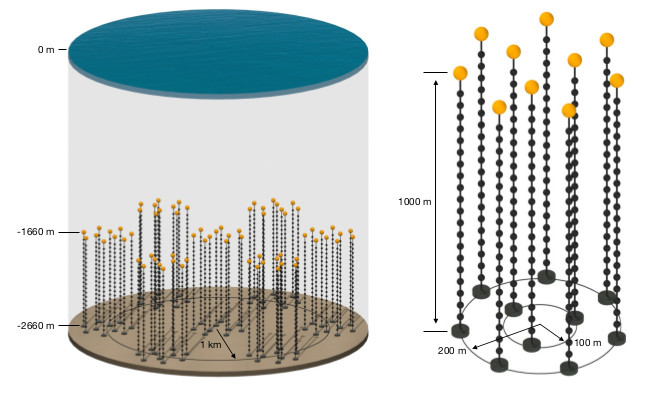
\includegraphics[width=12cm]{./Figures/PONEv0_-23_design.jpg}
  \caption{Left: Proposed full detector of the P--ONE detector. Right: Proposed array for the Explorer deployment of P--ONE.}
  \label{fig:pone_geo}
\end{figure}

With the current proposed geometry, the detector will be incredibly sensitive to horizontal incoming high energy muons from astrophysical neutrino sources \cite{pone}. 

\section{Detectors}
Similar to previously constructed neutrino telescopes, P--ONE will primarily use Vavilov--Cherenkov Radiation from leptons produced through neutrino interactions. This electromagnetic radiation is then detected through highly sensitive optical modules containing photomultiplier tubes (PMTs).

\subsection{Photomultiplier Tubes}

A key part of any neutrino telescope is the detection mechanism, and in this community the PMT is synonomous with detector. The PMT is a vacuum--sealed photocathode with dynode and anodes above connector pins \cite{ham}. The primary mechanism of a PMT is the photoelectric effect from a photon hitting the photocathode \cite{pmt_hist}. This ejected electron than travels and collides with another cathode, which results in more elctrons being ejected. This results in a cascade of electron showers along the dynodes and anodes amplifying the signal before it reaches the connector pins \cite{pmt_hist}. Through this method the PMT can produce large signals at the single photon level, yet is only sensitive to a particular range of frequencies/wavelengths of light \cite{pmt_hist}.

In particular, PMTs are generally sensitive to wavelengths anywhere as low as 100 nm to as high as 500 nm depending on the material of the photochathode \cite{ham}. Another property of PMTs to note is the Quantum Efficiency (QE), which is defined as the ratio of photoelectrons emitted by the photocathode to the number of incident photons \cite{ham}. Thus, QE defines the probability an incident photon causes a signal. The QE is dependent upon the photocathode and varies with the incident photons wavelength, as different wavelengths carry different energies \cite{ham}.

In contrast to QE, the Dark Current (Dark Noise) is the reporting by PMTs of light even in completely dark environments \cite{ham}. According to the Hamamatsu handbook \cite{ham}, a number of reasons can be the cause for this misfiring in PMTs including (but not limited to) thermionic emissons, internal current leakage, scintillation from glass envelope and radiation sources. One can minimize the effect from these sources, such as reducing the temperature to limit the thermionic emissions \cite{ham}.

The final aspect of PMTs we discuss is afterpulsing, the small pulses observed after the arrival of a signal \cite{ham}. The quick afterpulses (within nano--seconds) can usually be attributed to scattering of electrons on the first dynode \cite{ham}, while later afterpulses (within microseconds) can be the result of positive ions from the ionization of residual gases in the tube \cite{ham}.

The PMT is an incredibly technical piece of hardware, and characterizing each PMT is important to understanding the detector as a whole. 

\subsection{Digital Optical Modules}

In IceCube, the Digitial Optical Module (DOM) is a module containing a ten--inch PMT supported by coupling gel, the high voltage generator, an LED flasher board for calibration, and the mainboard used for analog and digital signal processing \cite{icecube_pmt,icecube} which allows for near--autonomous function. P--ONE will be adopting this approach for detector construction.

\begin{figure}[H]
  \centering
  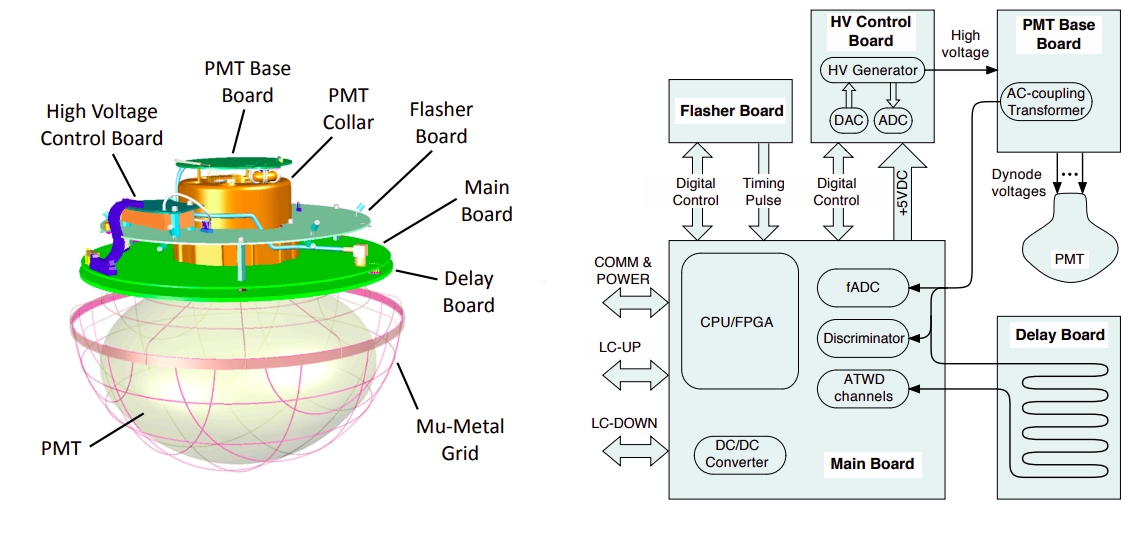
\includegraphics[width=.9\textwidth]{./Figures/icecube_dom.png}
  \caption{A diagram and schematic of the IceCube DOM.}
  \label{fig:ice_dom}
\end{figure}

Figure \ref{fig:ice_dom} shows a diagram of the IceCube DOM along with a schematic of the electronics that are on board. 


\subsection{mDOMs}

A proposed redesign of the IceCube DOM to increase the granularity of light detection is the multi--DOM (mDOM). In place of one large PMT, multiple smaller PMTs can line the same space and provide coverage at the cost of gaps between detectors. The benefit being that individual hits on the smaller PMTs can provide extra information using the acceptance angle and directionality of that particular PMT \cite{mpmt}. Moreover, in theory this can also reproduce the standard DOM data as the signal collected by a single PMT in the array can be collected and treated as a hit for the entire DOM. This gives the mDOMs a felxibility that isn't present for standard DOMs. In IceCube the standard DOMs use a ten--inch diameter PMTs \cite{icecube}, where the mDOMs would use up to 24 three--inch diameter PMTs \cite{mpmt}. Another point to note is that the photocathode area plays an important role in the amount of photons that can be detected, and hence the amount of information that can be collected from an event \cite{icecube}. 

\section{Strings for Absorption length in Water}

The pioneer (sometimes referred to as pathfinder) mission for P--ONE is the STRings for Absroption length in Water (STRAW) and its follow up STRAW--b, which were deployed in 2018 and 2020 respectively. The purpose of these missions was to test the technical details of running an experiment like P--ONE, in particular the hardware limitation, to provide data to measure the attenuation length of light in water for light in wavelengths between 350 nm and 600 nm, characterize the bioluminescence of deap--sea living organisms and the $^{40}$K dissolved in the salty water \cite{straw}.

\begin{figure}[H]
  \centering
  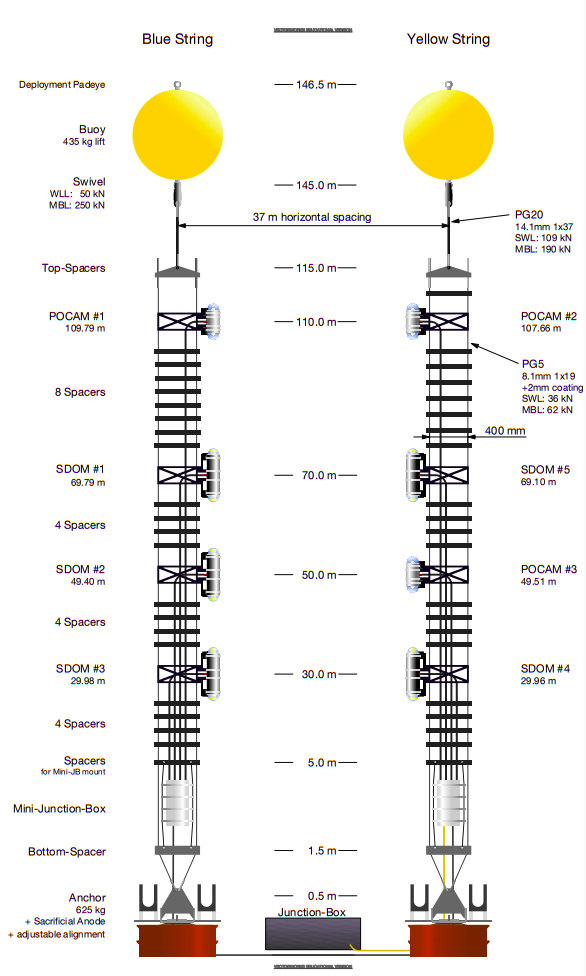
\includegraphics[width=.7\textwidth]{./Figures/STRAW.png}
  \caption{A diagram of the full STRAW setup including distances \cite{straw}.}
  \label{fig:straw}
\end{figure}

The basic design of STRAW, as shown in Figure \ref{fig:straw}, is the same as that of standard neutrino telescopes; using PMTs for detecting photons and calibrating light emitting sources on mooring lines to collect data \cite{straw}. In this particular case STRAW uses two vertical mooring lines with $3^{\prime\prime}$ PMTs and Precision Optical Calibration Modules (POCAMs) for the calibration sources \cite{straw}, which provide isotropic and short pulsed flashes of light. The POCAMs are the powerhouse of this endeavour. They offer an adjustable source of intense isotropic light ($\mathcal{O}(10^{9})$) \cite{pocam}. The glass hemispheres that house the POCAMs provide a transmissivity of $>95\%$ in the range between 350nm and 600nm \cite{pocam}. The attenuation length $L_{T}$ in water can be determined using the known photon intensity $N_{0}$, the wavelength from the POCAM flashes and the distance $r$ to each particular PMT with effective collection area $A_{\text{det}}$ measuring an intensity $N(r)$ \cite{straw}. This yields
\begin{equation}
  N(r) = \frac{N_{0}}{4\pi r^{2}}\exp\left(-\frac{r}{L_{T}}\right)A_{\text{det}}\, .
\end{equation}
The expected maximum value of absorption length is around 50 meters, so the STRAW geometry has been chosen to cover the ranges between 20 m and 90 m \cite{straw}. Some of the geometry choices were purely due to technical limitations, such as the maximum safe cable lengths to minimize data loss \cite{straw}, while others were to preserve some form of symmetry between modules \cite{straw}.

\section{Ocean Networks Canada}

The construction and implementation of P--ONE is supported by Ocean Networks Canada (ONC), an oceanography observatory with a vast network monitoring the west and east coasts of Canada along with the arctic \cite{onc}. Situated at the University of Victoria, ONC uses cabled observatories, remote control systems and interactive sensors for data collection and evidence--based decision--making \cite{onc}. 

\begin{figure}[h]
  \centering
  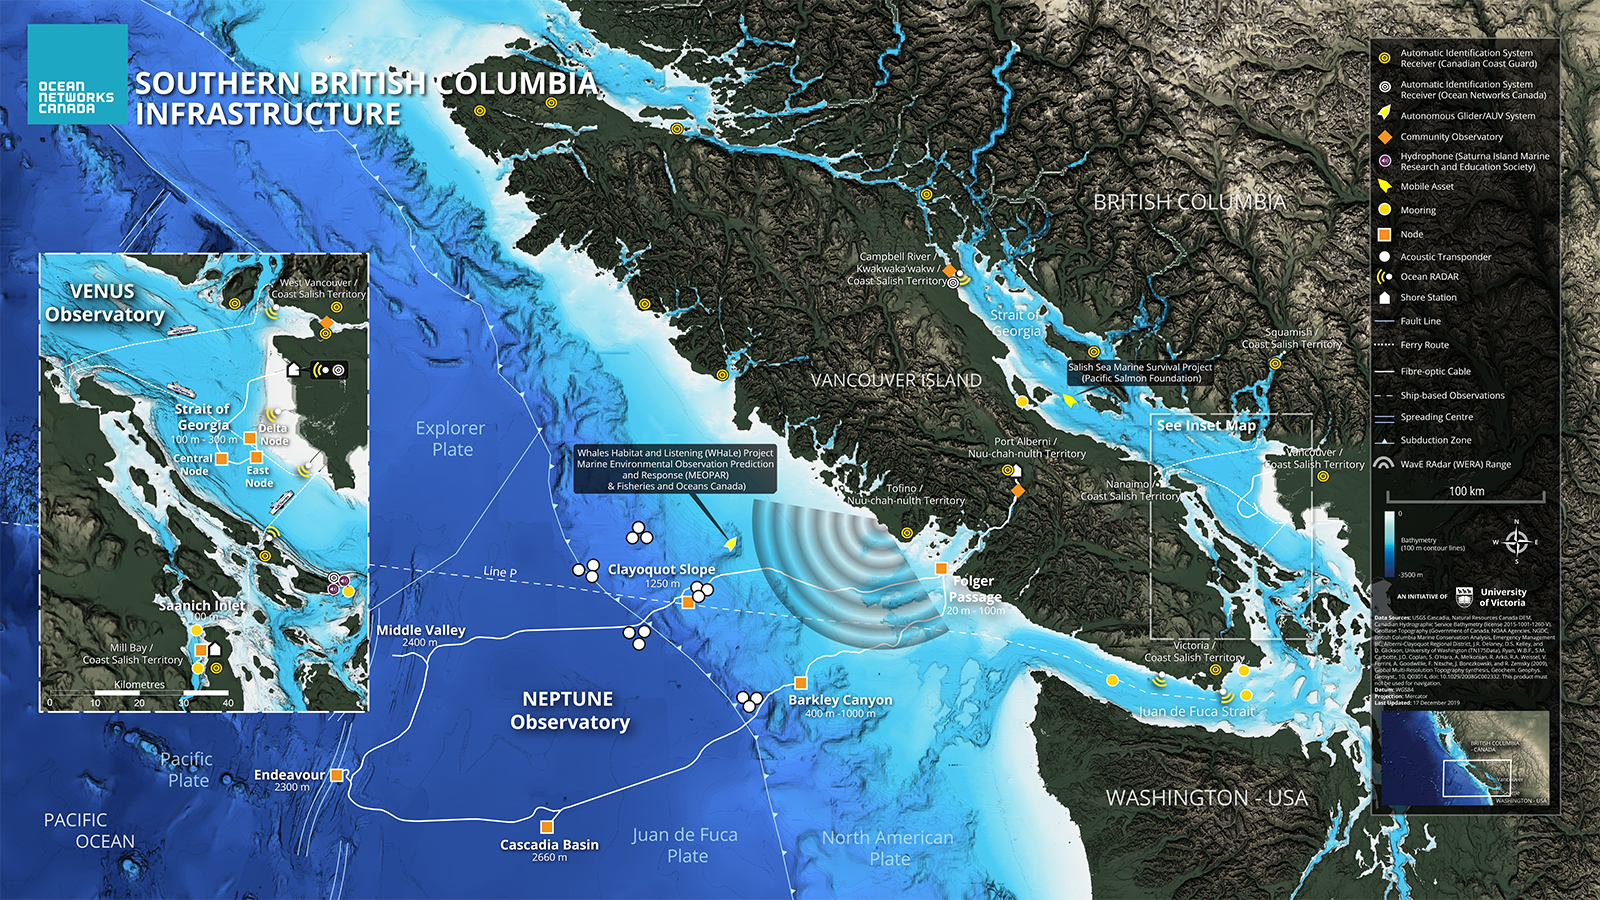
\includegraphics[width=.9\textwidth]{./Figures/western_infrastructure.png}
  \caption{A diagram of the Ocean Networks Canada Western Infrastructure for monitoring the Pacific Ocean. This contains the NEPTUNE and VENUS observatories. Source \cite{onc}.}
  \label{fig:west_inf}
\end{figure}

The west coast observatory, shown in Figure \ref{fig:west_inf}, is comprised of the 800--km NEPTUNE observatory and the nearly 50--km VENUS observatory \cite{onc}, with the NEPTUNE observatory housing the proposed site of P--ONE at the Cascadia Basin. The Cascadia Basin, as seen in Figure \ref{fig:casc}, is a heavily sedimented abyssal plain located 2660 meters below sea level \cite{onc}. Though the environment seems inhospitable, with temperatures below 2$^{\text{o}}$, high--pressure, and a distinct lack of light, one can still find organisms highly adapted to the extreme environment \cite{onc}. 

\begin{figure}
  \centering
  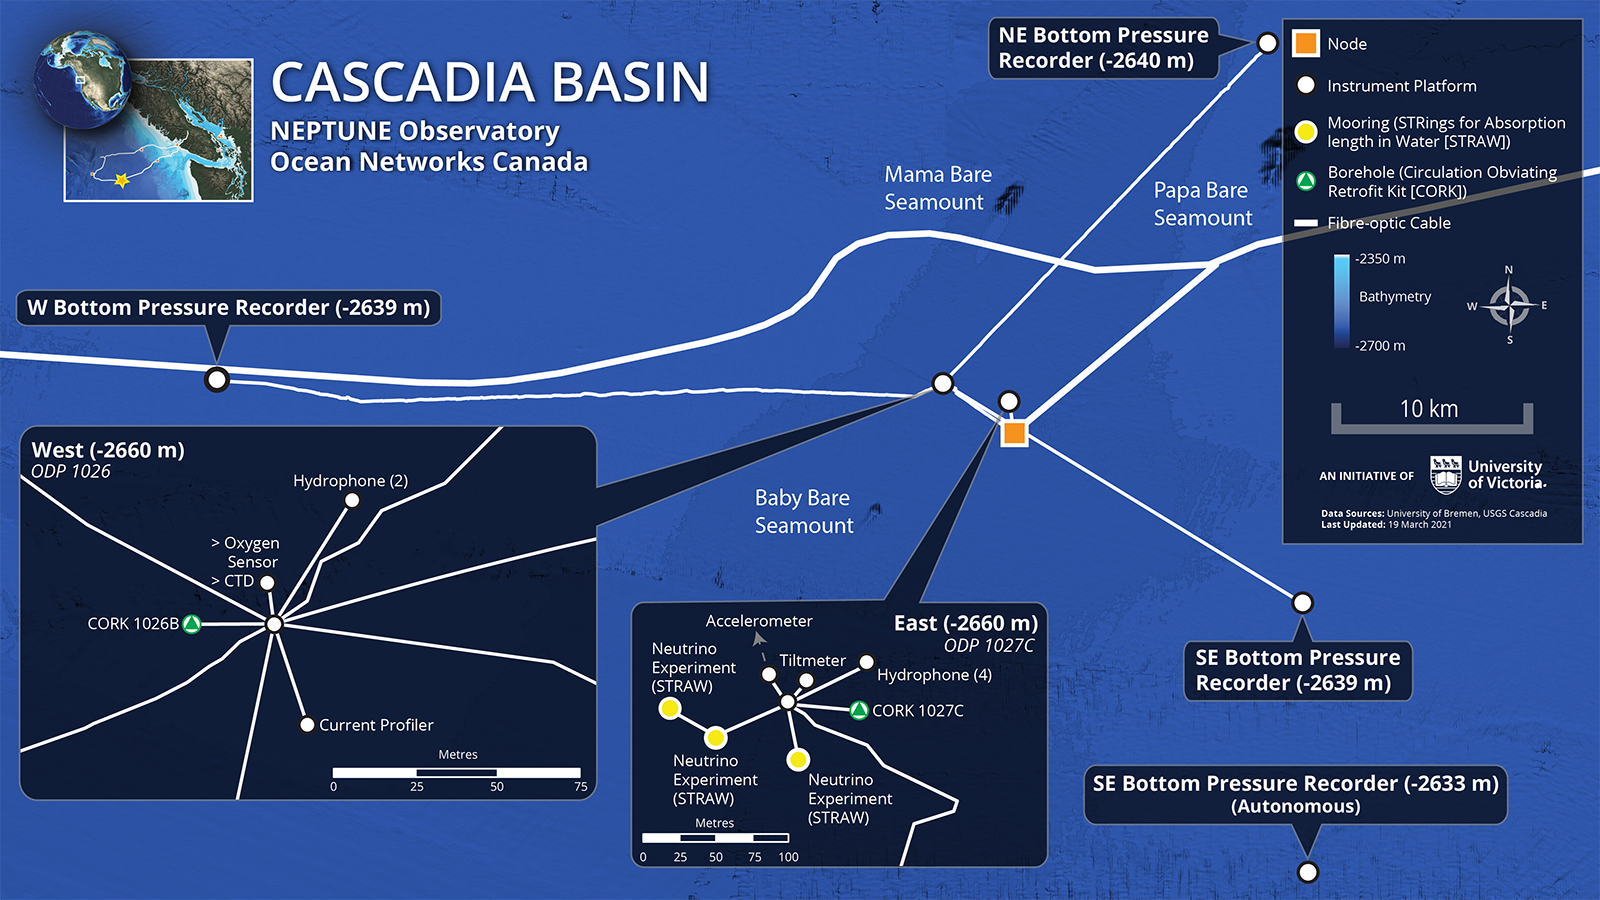
\includegraphics[width=.9\textwidth]{./Figures/cascadia_basin.png}
  \caption{Diagram of the Cascadia Basin, the site of the upcoming P--ONE experiment and current site of the pathfinder STRAW. Source \cite{onc}.}
  \label{fig:casc}
\end{figure}

This biodiversity results in the potential background of bioluminescence \cite{pone,onc,biolum,biolum_rec}. Bioluminesence is the emission of visible light by living organisms due to natural chemical processes used by a wide range of species \cite{biolum}. Some studies show that 75\% of all organisms larger than 1 cm occurring below the surface down to 4000 m depth are capable of bioluminescence \cite{biolum_rec}. Due to evolutionary advantages, most bioluminescent organisms emit light between 440 nm and 540 nm, which also has the largest absorption length in water \cite{biolum}. The amount of photons emitted can also vary significantly from $10^{3}$ for bacterium to $10^{12}$ photons from some fish \cite{biolum}. There are efforts being put together to understand and characterize this background in order to be better prepared for when the detector is installed.




\chapter{Simulation}

As P-ONE has only deployed the Pathfinder missions thus far, including STRAW and STRAWb, the data used in this thesis is primarily simulated. In particular, the data needs to be usable to test and build a reconstruction algorthim for muon-neutrinos. This means simulating muon tracks. For this reason, we lightly cover the simulation process used to produce data including the pre-existing IceCube Framework, Simulating Neutrinos, Simulating Muons and the Detector Response. 

\section{IceCube Framework}

The software framework already exists from IceCube, and in order to minimize the amount of new code needed to simulate P-ONE it is simplest to use the IceCube software. In particular, the software documentation is readily available \cite{icetray} and referred to as IceTray. This is meant to be a full framework capable of simulating, reconstructing and analysis all in one \cite{icetray}. For the purposes of P-ONE, we wish to only use the simulation subset of the framework as it is primarily made using open-source software, and hence can avoid potential proprietary issues.

The bulk of the code is written in C++ with the goal of being modular. This means that rather than writing scripts that call functions or classes that are pre-existing, the code is designed so that there is a single steering script that calls modules to run tasks including the simulation of muons or neutrinos, and including geometry files. Modules can be added by users as well to then be included in the steering scripts. The code has also been wrapped using Python so that modules can be reached via python scripts, and hence steering scripts can be written in Python. For this reason, Python is the language of choice for the purposes of this work.

\section{Simulating Neutrinos}

The sofware used to generate neutrinos is the very aptly named Neutrino-Generator (NuGen) \cite{icetray}. This is code written in IceTray based off of the All Neutrino Interaction Generator (ANIS), a high energy neutrino generator used for neutrino telescopes. NuGen has the capabilities of preparing and injecting a neutrino and interacting along the way if they so happen, and then forcing an interaction in the detector. NuGen can also produce secondaries. However, NuGen does not propogate photons nor charged leptons. This is saved for PROPOSAL and CLSim, where the former is used to propogate charged leptons and the latter is used to produce and propogate photons in a parallel manner (if using GPUs). 

\section{Simulating Muons}

Do we talk about Muon Gun or Cosmic Muons? Currently only Cosmic Muons are being used but both could be used.

\section{Detector Response}

This has to include the detector geometry (GCD) files, the DOMs, and efficiency...?


\chapter{Reconstruction}

A telescope is only as good as it's ability to identify distinct sources. In the case of a neutrino telescope this translates directly to how well observed events can be reconstructed for the direction of high energy events. IceCube uses several reconstruction methods \cite{icecube} and has several data quality checks it must go through before a result is given any weight. Similarly, ANTARES has had years of work put into the reconstruction software in order to reach the accuracies it can now \cite{antares}. To set the context for reconstructions, we need to first understand the data that is collected and how it appears. 

\section{Geometry of a Single Hit}

At first thought, it may sound simple to try and reproduce the tracks that produce the light one would observe in neutrino detectors, but upon considering the data that is aquired the true complexity is revealed. To see this, we consider first the geometry of a single hit to see what the data would look like. Referring to Figure \ref{fig:ghit}, we consider a muon track that is infinite in length, which is a safe approximation assuming a sufficient energy of the neutrino relative to the size of the detector. Specifically we can parameterize the track with
\begin{equation}\label{eq:track}
  \vec{u}(t) = \vec{x} + ct\vec{v}\, ,
\end{equation}
where $\vec{x}$ is the vertex, $\vec{v}$ is the direction the muon is travelling in, $t$ is the time parameter, and finally $c$ is the speed of light, which again for sufficiently high energy muons is a good approximation for the speed. Looking at the $i^{\text{th}}$ DOM located at a position $\vec{r_{i}}$, it is easy to see there must be a closest approach position for the track, $\vec{p}_{i}$, and emission point of a photon given there is a direct hit on the DOM, located at $\vec{q}_{i}$. The photon is emitted at a cherenkov angle of $\theta_{c}$, which is as described in equation \ref{fig:cher_angle}. 


\begin{figure}
  \centering
  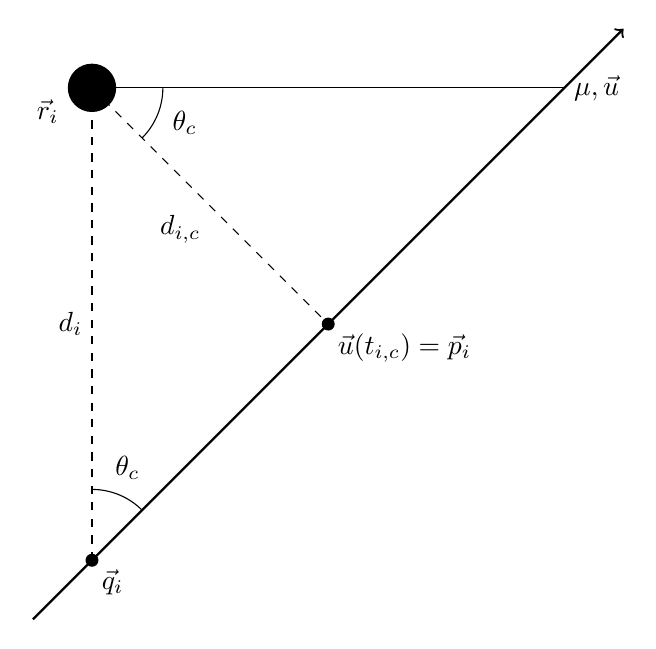
\begin{tikzpicture}[scale=3]
    % Closest point to DOM
    \node [below right] at (0,0) {$\vec{u}(t_{i,c}) = \vec{p}_{i}$};
    \node [below left] at (-0.5, 0.5) {$d_{i,c}$};
    \draw[fill] (0,0) circle [radius=0.025];
    \draw [dashed] (-1,1) -- (0,0);
    % Muon Travel line
    \draw [thick, ->] (-1.25,-1.25) -- (1.25,1.25);
    \node [right] at (1,1) {$\mu, \vec{u}$};
    % Emission point
    \node [below right] at (-1,-1) {$\vec{q}_{i}$};
    \node [above] at (-0.85, -0.7) {$\theta_{c}$};
    \draw[fill] (-1,-1) circle [radius=0.025];
    \draw (-1,-0.7) arc [radius=0.3, start angle=90, end angle=45];
    % DOM
    \node [left] at (-1.1,0.9) {$\vec{r}_{i}$};
    \draw[fill] (-1,1) circle [radius=0.1];
    % Emission Photon
    \node [left] at (-1,0) {$d_{i}$};
    \draw [dashed] (-1,-1) -- (-1,1);
    % Light Wavefront
    \node [right] at (-0.7,0.85) {$\theta_{c}$};
    \draw (-1,1) -- (1,1);
    \draw (-0.7,1) arc [radius=0.3, start angle=0, end angle=-45];
  \end{tikzpicture}
  \caption{Drawing of muon track and Vavilov-Cherenkov Radiation hitting a single DOM.}
  \label{fig:ghit}
\end{figure}

The next step is to consider the information we know about the DOMs. In particular, the direction of the DOM will determine its angular acceptance giving information on whether or not particular photons can actually reach the DOMs, and the time at which photons are detected. Moreover, light can scatter and may not travel a direct path, so the distance $d_{i}$ also becomes an important parameter to consider. Any sophisticated reconstruction technique will require these parameters to produce reliable results, and hence are important to both understand and compute given a track. Hence, we first attempt to discuss the method for computing these parameters given a DOM position and track.

Assuming a track as given in equation \ref{eq:track}, and that we know the closest approach position at $\vec{p}_{i}$ for a DOM at $\vec{r}_{i}$, then we can easily compute $d_{i,c} = |\vec{p}_{i} - \vec{r}_{i}|$. Then, using the closest approach distance,
\begin{equation}\label{eq:dist}
  d_{i} = \frac{d_{i,c}}{\sin\theta_{c}}
\end{equation}
will describe the distance the photon travels. To get the emission point of the photon $\vec{q}_{i}$, we know that $s_{i} = d_{i}/\tan\theta_{c}$ and that the corresponding time would be $t_{s} = s/c$. Then we see that
\begin{equation}
  \vec{q}_{i} = \vec{p}_{i} - ct_{s}\vec{v} = \vec{p}_{i} - s\vec{v}\, ,
\end{equation}
where $\vec{p}_{i} = \vec{u}(t_{i,c}) = \vec{x} + ct_{i,c}\vec{v}$, and so
\begin{equation}\label{eq:emit}
  \vec{q}_{i} = \vec{x} + (ct_{i,c} - s)\vec{v}\, .
\end{equation}
It is important to note that the distance term $s$ is negative in equation \ref{eq:emit} due to the photon being emitted before the track will be closest to the DOM.

Now, we know where the emission point is and we know the distance $d_{i}$ from equation \ref{eq:dist}. Now, we want to compute the geometric time, as in the time we would expect the photon to arrive at the DOM from our proposed track. To predict this time, we need a reference along the track, and the vertex $\vec{x}$ is a natural choice for this. Then, we know that
\begin{equation}
  t_{\text{geo}} = t_{d} + t_{x}
\end{equation}
where
\begin{equation}\label{eq:travel_time}
  t_{d} = \frac{d_{i}}{c_{n}}\, , \hspace{2em} \& \hspace{2em} t_{x} = \frac{(\vec{q}_{i} - \vec{x})\cdot\vec{v}}{c}\, .
\end{equation}
The former is the time it takes for the emitted photon to travel directly to the DOM, with $c_{n}$ being the group velocity of light in water, and the latter is the time it takes for the muon to travel from the vertex to the emission point. It is important to note that in the second term of equation \ref{eq:travel_time}, the numerator makes sure that the travel time has the correct value. Since the vertex $\vec{x}$ is not physical, and is mearly a reference point for the purposes of this thesis, it is possible for this to be after the emission point. In that case, the value $t_{x}$ would have to be negative, and this projection onto the direction vector of the track ensures this. Now, given that we know the time at which the muon is at the vertex, we can shift this travel time accordingly to a shifted $t_{\text{geo}}$ that will now be comparable to the time that the DOM reports, $t_{\text{obs}}$. The parameter of importance then is the residual time, defined as
\begin{equation}
  t_{\text{res}} = t_{\text{obs}} - t_{\text{geo}}\, ,
\end{equation}
as it will vaguely inform of the difference between the geometric guess track and the true track. 

\begin{figure}
  \centering
  \begin{tikzpicture}[scale=3]
    % Origin
    \node [above left] at (-2.5,0.5) {$\mathcal{O}$};
    \draw [fill] (-2.5,0.5) circle [radius=0.05];
    % x and r vector
    \node [below left] at (-1.75,-0.25) {$\vec{x}$};
    \node [above left] at (-1.75,0.75) {$\vec{r}$};
    \draw [->] (-2.5,0.5) -- (-1.017,-0.982);
    \draw [->] (-2.5,0.5) -- (-1,1);
    % Closest point to DOM
    \node [below left] at (-0.5, 0.5) {$d_{c}$};
    \draw [fill] (0,0) circle [radius=0.025];
    \draw [dashed] (-1,1) -- (0,0);
    % Muon Travel line
    \node [right] at (1,1) {$\mu, \vec{u}$};
    \draw [thick, ->] (-1.25,-1.25) -- (1.25,1.25);
    % Emission point
    \node [below right] at (-0.5,-0.5) {$((\vec{r} - \vec{x})\cdot\vec{v})\vec{v}$};
    \draw [fill] (-1,-1) circle [radius=0.025];
    % DOM
    \draw [fill] (-1,1) circle [radius=0.1];
    % Emission Photon
    \node [left] at (-1,0) {$\vec{r} - \vec{x}$};
    \draw [->] (-1,-1) -- (-1,1);
  \end{tikzpicture}
  \caption{Drawing of a track with vertex and DOM labeled. The origin here is also marked to emphasize the vector notation and algebra. It is easy enough to see the vector algebra required to get the distance of closest approach through this diagram.}
  \label{fig:dic}
\end{figure}

The next step is to recall all these prior computations rely on the distance of closest approach ($d_{i,c}$) being known. To compute this, we need some geometric considerations with the vectors of the track, the DOM and the vertex. To visualize the vector algebra, we can introduce an origin from which the vectors can be drawn, in which case we get Figure \ref{fig:dic}. We see that the vector pointing to the vertex is $\vec{x}$ and the vector pointing to the DOM is $\vec{r}$, where the indices are dropped for convenience. Then, we see that a vector pointing from the vertex to the DOM can be defined by $\vec{r} - \vec{x}$. Next, we can find the projection of this vector along the track direction (which is already a unit vector) as being $(\vec{r} - \vec{x})\cdot\vec{v}$. Then, we see that we have two sides of a right angle triangle with the third missing side being the length $d_{c}$, so
\begin{equation}
  d_{c} = \sqrt{|\vec{r} - \vec{x}|^{2} - |(\vec{r} - \vec{x})\cdot\vec{v}|^{2}}\, .
\end{equation}

We now have a method of computing $d_{i,c}$, and thus computing $d_{i}$ and $t_{\text{res}}$ for each DOM given a proposed track $\vec{u}(t) = \vec{x} + ct\vec{v}$. It is important here to note the degrees of freedom that parameterizing a track have. The vertex provides four as it is a position in 3-dimensional space with a time attached. The direction provides two degrees of freedom, as it is a unit vector and can be parameterized using two angles and a unit length radius in spherical coordinates. This gives us six parameters in total that need to be computed to uniquely define an infinite track. 

We are now ready to consider different methods for computing these parameters. There are several software techniques that need to be applied before a result can be taken seriously, and usually this pipline begins with a simple and quick initial guess fit. 

\section{Linefit}

Any robust reconstruction method requires an initial guess (generally referred to as a seed) in order to be used, but getting this first guess can be non-trivial. Moreover, reconstruction pipelines can be incredibly sensitive to the initial guess and ensuring the quality of this fit is difficult in its own right. The standard method for a first guess in such situations is the linefit/linear fit. This is a simple track fit that minimizes the $\chi^{2}$ on the observed hits given in an event. As such, this fitting technique assumes that all hits on the DOMs are directly on the path of the muon track, which is a decent first approximation.

\begin{figure}
  \centering
  \begin{tikzpicture}[scale=5]
    % Drawing the x,y,z-t axis
    \node [right] at (1,0) {$t$};
    \node [above] at (0,1) {$x,y,z$};
    \draw [thick, ->] (0,0) -- (1,0);
    \draw [thick, ->] (0,0) -- (0,1);
    % Drawing the points to be fit
    \draw [fill] (0.1,0.4) circle [radius=0.025];
    \draw [fill] (0.2,0.2) circle [radius=0.025];
    \draw [fill] (0.4,0.4) circle [radius=0.025];
    \draw [fill] (0.6,0.7) circle [radius=0.025];
    \draw [fill] (0.8,0.6) circle [radius=0.025];
    \draw [fill] (0.95,0.85) circle [radius=0.025];
  \end{tikzpicture}
  \caption{Drawing of the position and time space with possible points $(x_{i},y_{i})$ that would be fit.}
  \label{fig:linfit}
\end{figure}

Under these approximations, we assume each spatial coordinate independent from the others. Then we can fit linearly in the projected two dimensional spaces of position and time: $x-t$, $y-t$ and $z-t$, where $t$, the time of the corresponding hit, is the independent variable. This way, the problem is reduced to fitting the equation $y=c_{1}x + c_{0}$ in each position and time space as seen in Figure \ref{fig:linfit}. From here, we need only apply $\chi^{2}$ minimization, which in the case of linear data fitting is exactly the method of least squares. In this scenario, if the data points are defined as $(x_{1},y_{1}), \dots, (x_{m},y_{m})$, then the solution that minimizes the $\chi^{2}$ will be
\begin{equation}
  \vec{c} = (X^{T}X)^{-1}X^{T}\vec{y}\, ,
\end{equation}
where
\begin{equation}
  \vec{c} =
  \begin{bmatrix}
    c_{0} \\
    c_{1}
  \end{bmatrix}
  \quad \& \quad
  X =
  \begin{bmatrix}
    1 & x_{1} \\
    1 & x_{2} \\
    \vdots & \vdots \\
    1 & x_{m}
  \end{bmatrix}
  \quad \& \quad
  \vec{y} = 
  \begin{bmatrix}
    y_{1} \\
    y_{2} \\
    \vdots \\
    y_{m}
  \end{bmatrix}\, .
\end{equation}
Once $\vec{c}$ is computed for each position and time space, the vertex position is estimated to be at $(c_{0,x}, c_{0,y}, c_{0,z})$ with direction $(c_{1,x}, c_{1,y}, c_{1,z})$, where the second subscript denotes the spatial component of the data that was used in the fit. 

% Can add charge section (make sure to credit Thomas in statement of originality)
\section{Likelihood}

A more robust technique for reconstructing potential muon tracks is a Maximum Likelihood Estimate \cite{llh_text}. In essence this is a statistically driven parameter fitting technique that allows for more complex modelling, such as the inclusion of the VC emissions. Specifically, if a single DOM observes data $\vec{x_{i}}$, then the probability of observing this data given track parameters $\vec{\theta}$ is described by a probability distribution $p\left(\vec{x_{i}}\bigr\rvert\vec{\theta}\right)$. Since this is true for each DOM in a given event, the likelihood distribution is defined as
\begin{equation}
  \mathcal{L}(\vec{\theta}) = \prod_{i=1}^{n}p\left(\vec{x_{i}}\bigr\rvert\vec{\theta}\right)\, ,
\end{equation}
where the indices are over all $n$ DOMs. The data, $\vec{x}$, can carry information such as the times, charges, and directionality of the hits. The varied parameters, $\vec{\theta}$, carry the information about the track including the direction, the vertex, the vertex time, and the energy. The parameters that maximize the distribution $\mathcal{L}(\vec{\theta})$ are the best guess for the track given this method.

Finding this maximum is generally non-trivial and a difficult problem. Computational limits motivate using more robust maximization techniques than full parameter searches, and generally these are techniques that use gradient driven methods. Due to this methodology, generally the solution proposed by the MLE is not the global maximum, and is usually a local maximum. The result of the maximization is thus heavily dependent upon the initial conditions and the exact method of fitting.

\subsection{Likelihood Function}

Though we understand the general theory for how the likelihood function will turn out, we still need an explicit form for $p\left(\vec{x_{i}}\bigr\rvert\vec{\theta}\right)$. This probability function could be made arbitrarily complex by attempting to account for every little physical detail, so we need to state the assumptions and physical processes that will be modeled. Using the fact that we know how to get the geometric time and direct distance that the emitted photon would travel before hitting the DOM given a guess track, the next step would be to account for the scattering and absorption of light. This seems like a small change, but has large repercussions in the probability distribution describing the data given a hypothesis track. IceCube uses the Pandel function \cite{phd_kai}, which explicitly takes the following form,
\begin{equation}\label{eq:pandel}
  \begin{split}
    p\left(t_{\text{res}}\bigr\rvert\vec{\theta}\right) = & \frac{1}{N(d)}\frac{\tau^{-d/\lambda}\cdot t_{\text{res}}^{d/\lambda - 1}}{\Gamma(d/\lambda)}\cdot \exp\left(-t_{\text{res}}\cdot\left(\frac{1}{\tau} + \frac{c_{\text{medium}}}{\lambda_{a}}\right) - \frac{d}{\lambda_{a}}\right)\, , \\
    N(d) = & e^{-d/\lambda_{a}}\cdot\left(1 + \frac{\tau \cdot c_{\text{medium}}}{\lambda_{a}}\right)^{-d/\lambda}\, ,
  \end{split}
\end{equation}
where $d$ is the photon travel distance, $\lambda$ is the scattering length, $\lambda_{a}$ is the absorption length, $\Gamma(x)$ is the Gamma function, $c_{\text{medium}}$ is the speed of light in water, and $\tau$ is an inverse time parameter for fitting \cite{phd_kai}. Given these parameters, which are physically motivated or fit using simulated data, the Pandel function gives the probability of observing a residual time for a hypothesis track. It is important to note here that $\vec{\theta} = (\vec{v}, \vec{x}, t_{\text{vertex}})$, where we have the track direction, vertex position and vertex time respectively.

The Pandel function favours positive residual times, so much so the probability has varying behavours as $t_{\text{res}}\to 0$. Figure \ref{fig:pandel} shows this behaviour 

\begin{figure}[H]
  \centering
  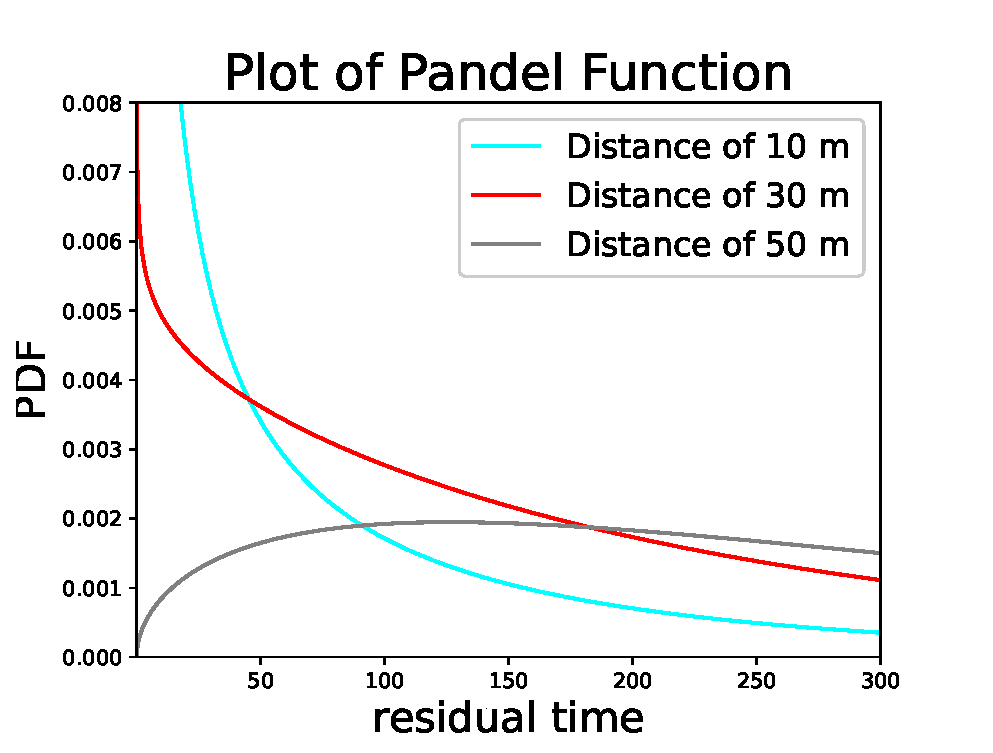
\includegraphics[width=12cm]{./Figures/pandel_plot.eps}
  \caption{A figure showing a plot of the pandel function over 300 nanoseconds with 10 meters, 30 meters and 50 meters of travel distances for the emitted light. }
  \label{fig:pandel}
\end{figure}

\chapter{Results}

\textbf{REMAKE PLOTS WITH EPS ONCE THEY ARE READY}

Having constructed the theory of the physics and computation, we are in a position to discuss the results that come about from these reconstruction efforts. To discuss these results, we consider the methods in which a reconstruction technique can be considered successful. The easiest, and most useful parameter to check is the direction. Comparing the reconstructed direction with the true direction is done by computing the solid angle between the directions. Computing this is simple; suppose the reconstructed direction is $\vec{u}$ and the true direction is $\vec{v}$, then the solid angle is
\begin{equation}
  \alpha = \arccos(\vec{u}\cdot\vec{v})\, ,
\end{equation}
where we are assuming the directions are normalized to unit length. This solid angle can then be used to fill a histogram of a large number of trials to build a distribution. 

\section{Linefit}

The simplest method for reconstruction that has been discussed is the linear fit using the method of least squares. In figure \ref{fig:alpha_linefit} we see that this method provides a pretty decent first guess for a direction. The angular resolution seems to peak around a three degree resolution, and slowly falls off as we get further away from the truth. 

\begin{figure}[H]
  \centering
  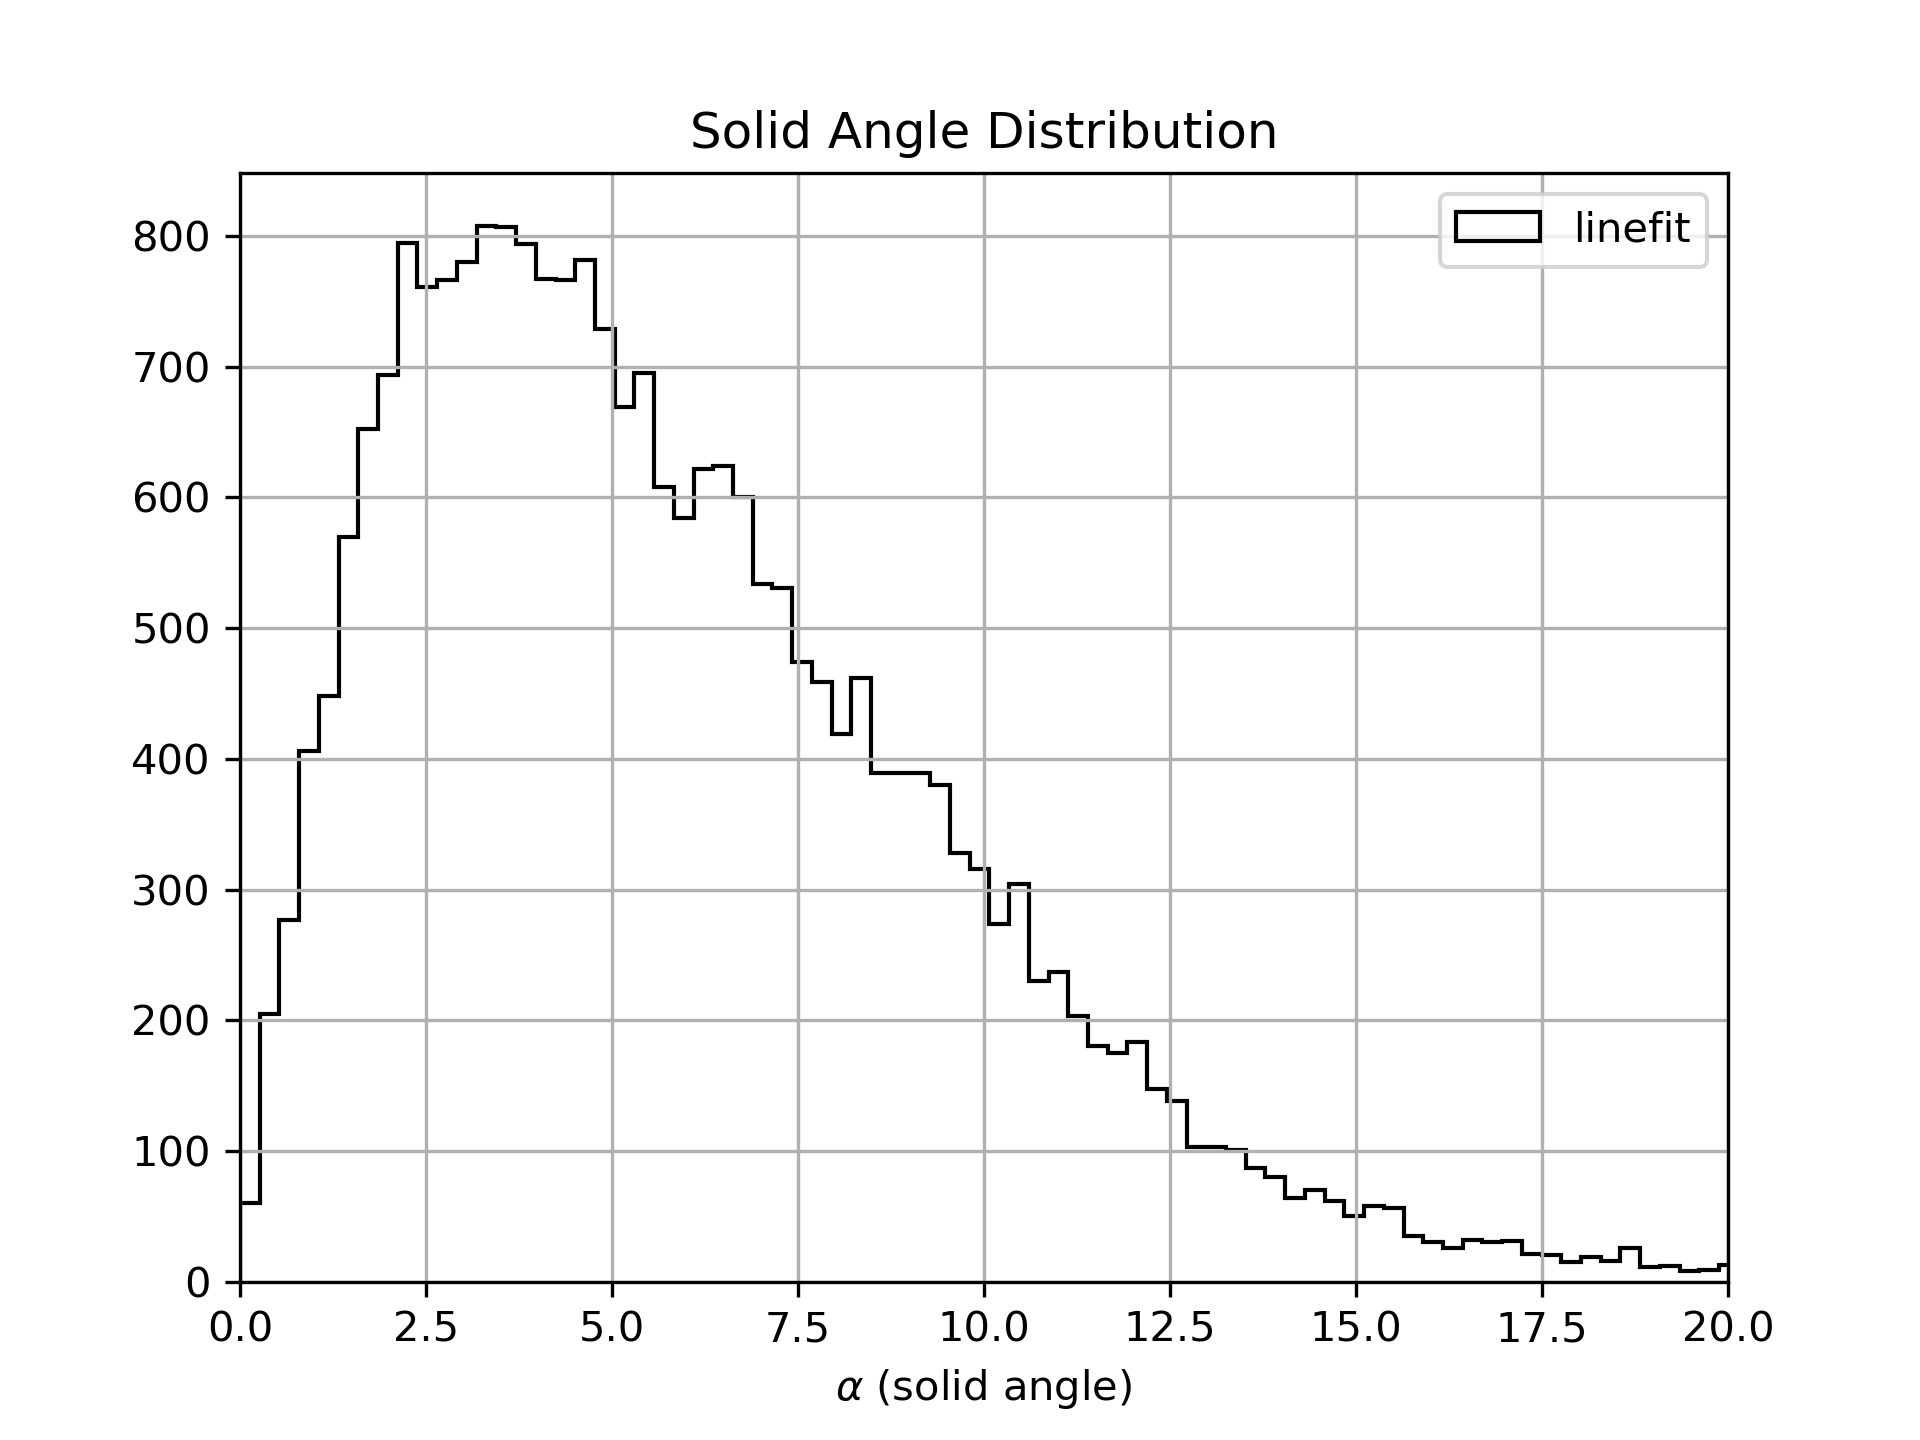
\includegraphics[width=12cm]{./Figures/reco_plots/alpha_dist_linefit_count.png}
  \caption{A distribution of the solid angles for reconstructed and true directions using the linefit method. The solid angle is given in degrees for clarity.}
  \label{fig:alpha_linefit}
\end{figure}

The quality of this reconstruction will inevitably affect the quality of the following reconstruction step, and as such should not be ignored. 

\section{Likelihood}

We can make a similar plot for the angular distribution of the reconstructed angle using the linefit as a seed to the likelihood algorithm. Looking at figure \ref{fig:alpha_llh} we see how well the likelihood reconstruction performs when using the linefit as a seed, but also how it compares to a perfect starting point, the true track information.

\begin{figure}[H]
  \centering
  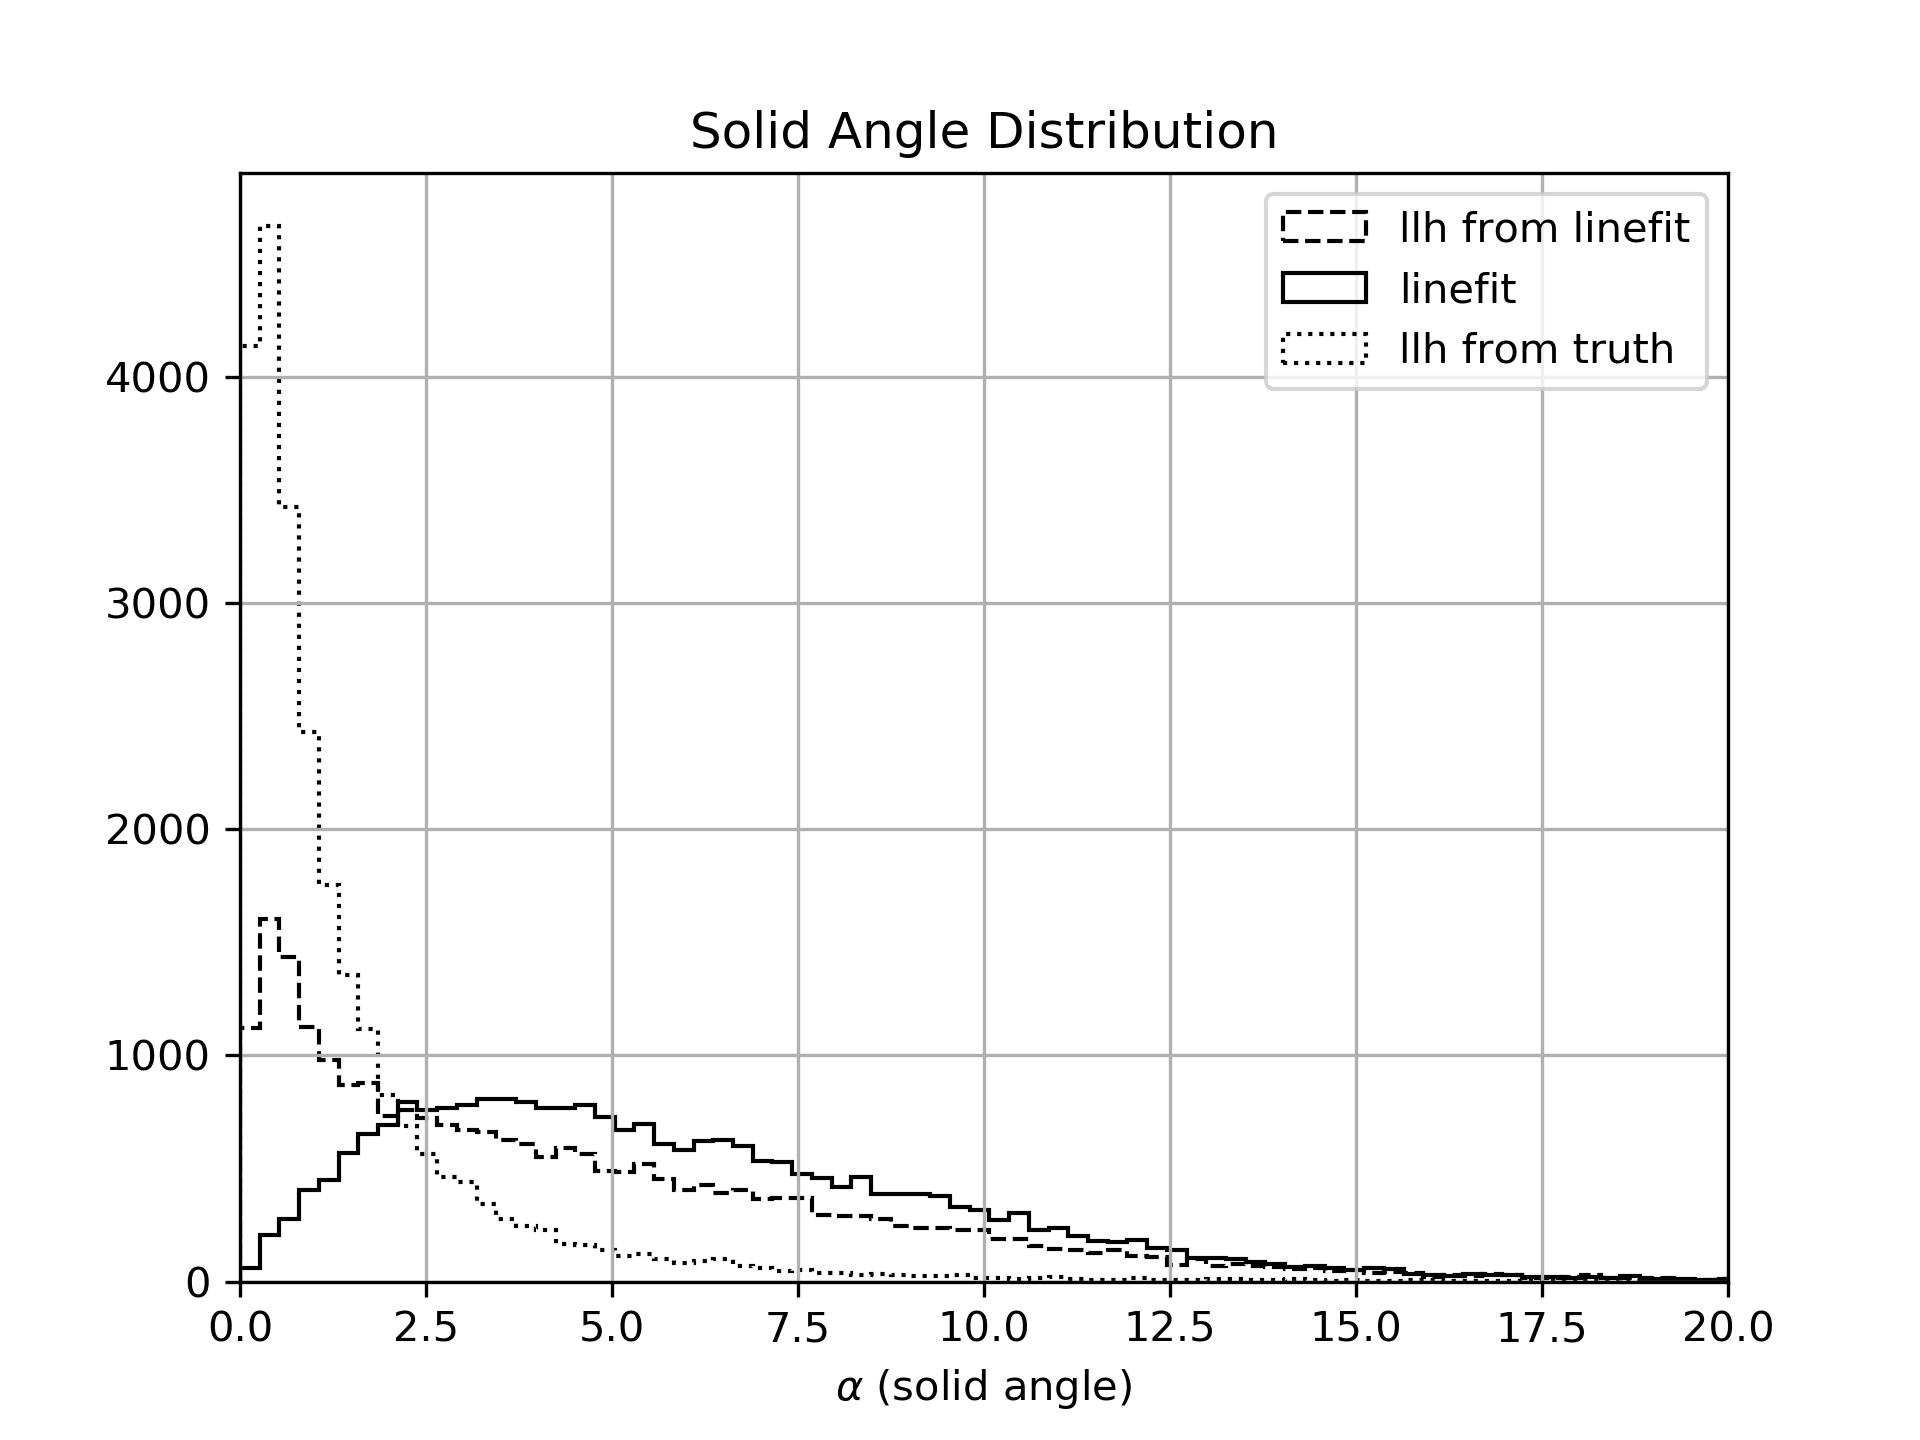
\includegraphics[width=12cm]{./Figures/reco_plots/alpha_dist_llh_count.png}
  \caption{A distribution of the solid angles for reconstructed and true directions using the likelihood method. The linefit reconstruction angular resolution is also plotted alongside a distribution for the likelihood given the true track as a starting point.}
  \label{fig:alpha_llh}
\end{figure}

Figure \ref{fig:alpha_llh} shows us that with perfect information, the likelihood reconstruction does pretty well. This effectively shows the upper limit to the performance of the reconstruction as it is, but also shows that there is plenty of room for improvement when starting at the linefit seed. It is relatively standard for reconstruction techniques to be highly dependent upon the initial conditions, as the technology used boils down to being a minimization of a multiparameter space. This effect is in full swing when we compare the two starting conditions, which emphasizes that another path to improving the reconstruction would be to improve the initial guess.

This resolution plot can also be represented by plotting the difference in the directional coordinates. As the directions are length one, we can seperate the azimuthal ($\phi$) and zenith ($\theta$) errors. Then, plotting the difference between the true azimuth/zenith and the reconstructed azimuth/zenith leads to figure \ref{fig:alpha_llh_sep}. 

\begin{figure}[H]
  \centering
  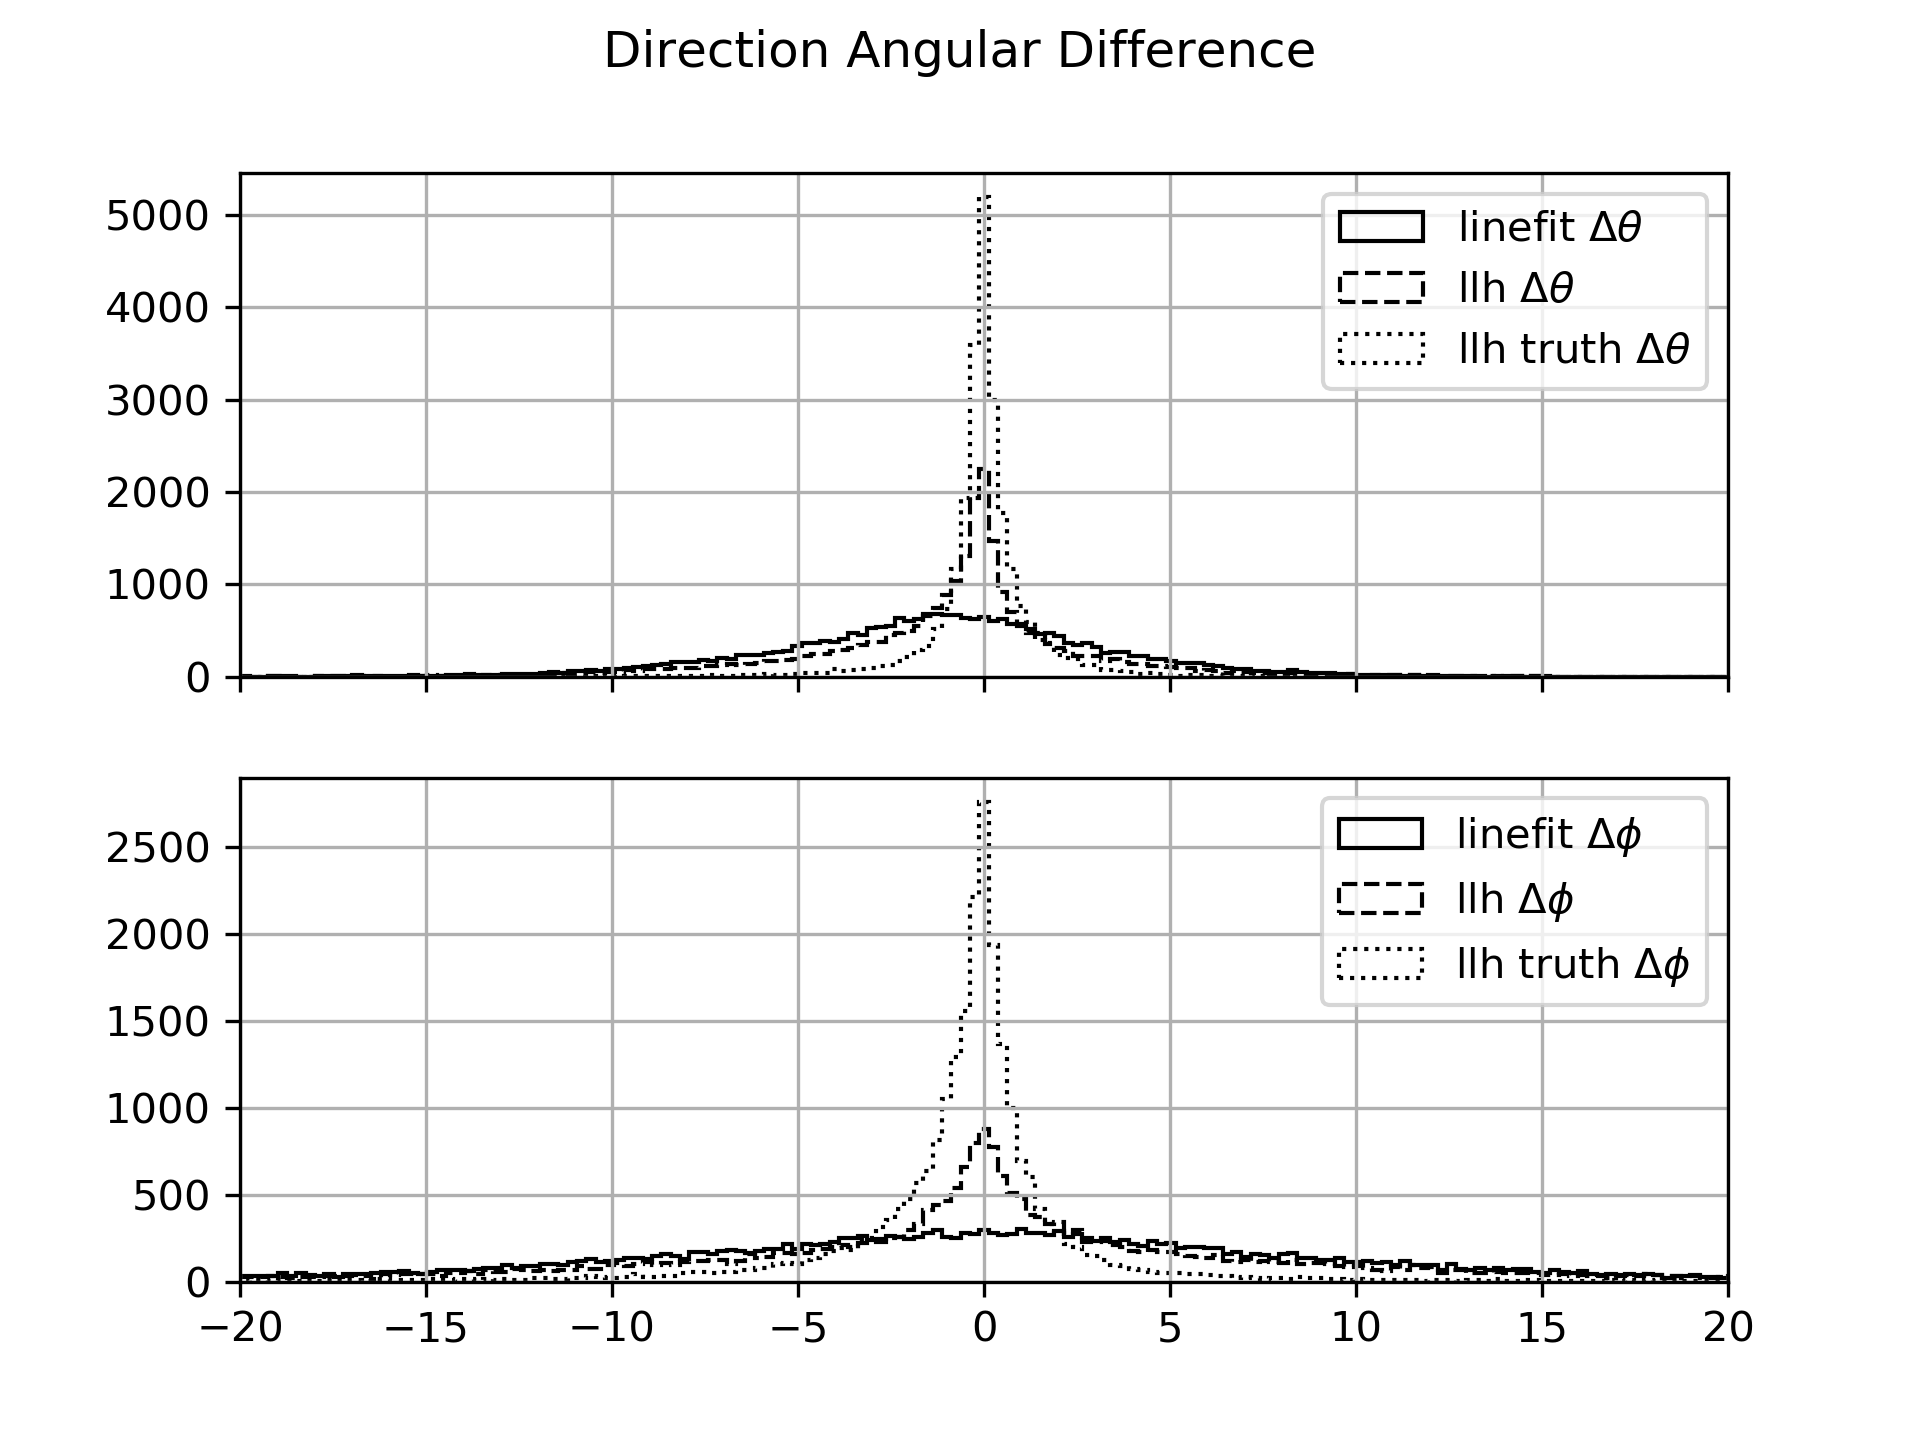
\includegraphics[width=12cm]{./Figures/reco_plots/angular_diff_dir.png}
  \caption{A distribution of the solid angles for reconstructed and true directions using the likelihood method seperated into zenith and azimuth components in degrees. \textbf{Above:} The zenith component distribution where $\Delta\theta = \theta_{\text{true}} - \theta_{\text{reco}}$ in the reconstruction process. \textbf{Below:} The azimuth component distribution where $\Delta\phi = \phi_{\text{true}} - \phi_{\text{reco}}$ in the reconstruction process.}
  \label{fig:alpha_llh_sep}
\end{figure}

The reconstruction still shows a similar shape that that observed in figure \ref{fig:alpha_llh}, as clearly the angular resolution in highly initial condition dependent. There is something of note in the zenth plot though ($\theta$), as there is a slight skewing towards negative $\Delta\theta$ values when using the linefit. This is due to the way the detector is simulated, since the current setup assumes IceCube-like DOMs which only face downward. As linefit is ignorant to the actual method in which light is emmitted from the track, this introduces a degeneracy in the fit that can push linefit towards a particular direction.

The resolution in the zenith angle seems to be slightly better than that of the azimuthal, which can be attributed to the geometry of the detector. In particular, the current geometry assumes vertical lines of detectors, which would expectedly perform better. These plots are in fact excellent for attempting to understand the effects of the geometry of the detector.

To test which initial parameter most affects the reconstruction, I started the reconstruction seed from two different initial states; fixing the starting vertex at the truth, and fixing the starting direction in the true direction. Using these initial conditions, a plot similar to figure \ref{fig:alpha_llh} could be created, and is in figure \ref{fig:alpha_llh_test}. As can be seen from the legend, there are a couple of variable seeds in this distribution, and the results seem to point towards the vertex resulting in the largest improvement in the resolution. This can come off as a bit surprising, especially when the parameter that is being plotted against is the direction resolution. The improvement does tell us where we need to improve the initial guess, and focusing on an improved vertex for the initial seed seems to be the way to go.

\begin{figure}[H]
  \centering
  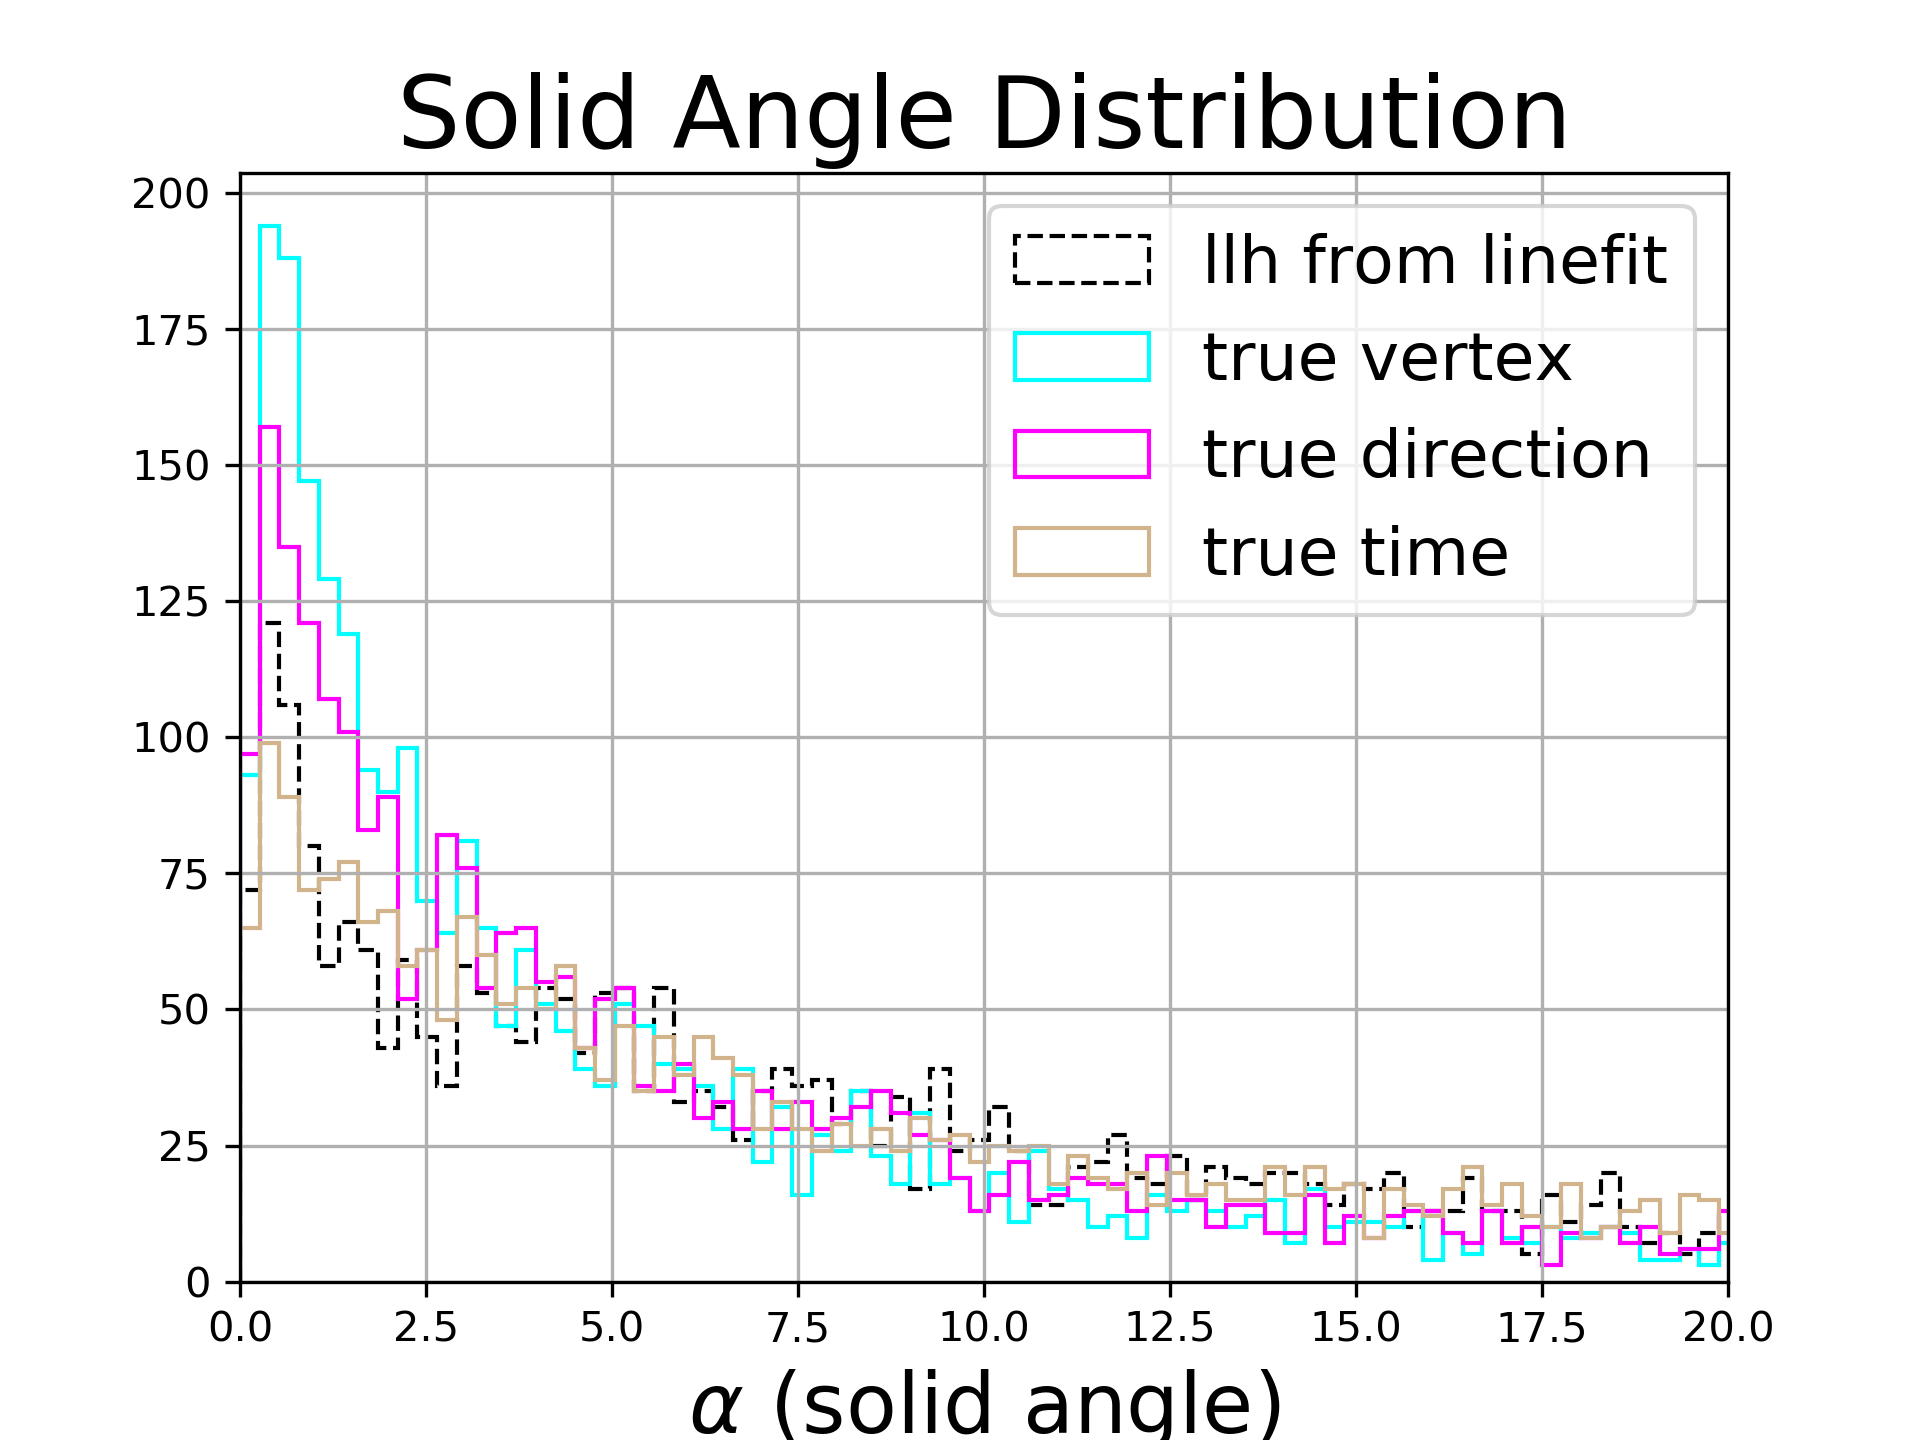
\includegraphics[width=12cm]{./Figures/reco_plots/alpha_dist_llh_seedcomparison.png}
  \caption{Similar to the distribution in figure \ref{fig:alpha_llh}, the angular resolution is plotted in degrees into a histogram. Here the initial starting conditions are grouped into the true vertex, true direction and only linefit, where the former are given linefit parameters for the remaining parameters.}
  \label{fig:alpha_llh_test}
\end{figure}

To get a better idea of how the plots in Figure \ref{fig:alpha_llh_test} and Figure \ref{fig:alpha_llh} compare, we can make a simple table to look at the percentage of events that are below certain cut-off angular resolution values. In Table \ref{tab:alpha_comp} we see these exact percentages for angular resolutions below $0.1^{\circ}$, $0.5^{\circ}$, $1^{\circ}$, $5^{\circ}$, and $10^{\circ}$ from the true direction. Comparing the values, we see that the largest relative increases in the percentages seem to occur between linefit and the standard likelihood reconstruction and going to the likelihood reconstruction using the truth as a seed. Looking at the resolutions below $0.1^{\circ}$, $0.5^{\circ}$, and $1^{\circ}$ the percentage of events increase by an order of magnitude between linefit and the standard likelihood method. This same jump occurs again when getting to the likelihood reconstruction using the truth as a seed. 

\begin{table}[H]
  \centering
  \begin{tabular}{|c|c|c|c|c|c|} 
    \hline
    $\mathbf{\alpha}$ & $\mathbf{0.1^{\circ}}$ & $\mathbf{0.5^{\circ}}$ & $\mathbf{1^{\circ}}$ & $\mathbf{5^{\circ}}$ & $\mathbf{10^{\circ}}$ \\
    \hline
    \textbf{line} & 0.02 & 0.39 & 1.54 & 24.25 & 50.76 \\
    \hline
    \textbf{llh} & 0.47 & 5.67 & 11.43 & 38.02 & 59.58 \\
    \hline
    \textbf{llhdir} & 0.69 & 7.60 & 15.70 & 50.11 & 70.54 \\
    \hline
    \textbf{llhvert} & 0.71 & 8.99 & 19.23 & 57.65 & 76.31 \\
    \hline
    \textbf{llhtrue} & 2.70 & 25.03 & 45.21 & 86.92 & 96.29 \\
    \hline
  \end{tabular}
  \caption{The labels `\textbf{line}', `\textbf{llh}', `\textbf{llhdir}', `\textbf{llhvert}', `\textbf{llhtrue}' refer to the linefit, likelihood, likelihood using the true direction seed, likelihood using the true vertex seed and likelihood using the truth as a seed reconstructions respectively. The values are given in percentage of events below the given $\alpha$ solid angle to the true direction.} 
  \label{tab:alpha_comp}
\end{table}

We can also check whether there is a correlation with the likelihood values and the reconstructed angular resolution ($\alpha$). To do so, we need a way to include both the final and initial likelihood values, as there can be a wide variety of ranges that a reconstruction can start and end at. For this reason, we consider plotting the ratio between the final negative loglikelihood value and the initial, $\ell_{f}/\ell_{i}$. Thus, a smaller value denotes a larger improvement in the likelihood value. On the other hand, any value above one denotes a drop in quality of fit. This plot is made in figure \ref{fig:alpha_llhratio_comp}.

\begin{figure}[H]
  \centering
  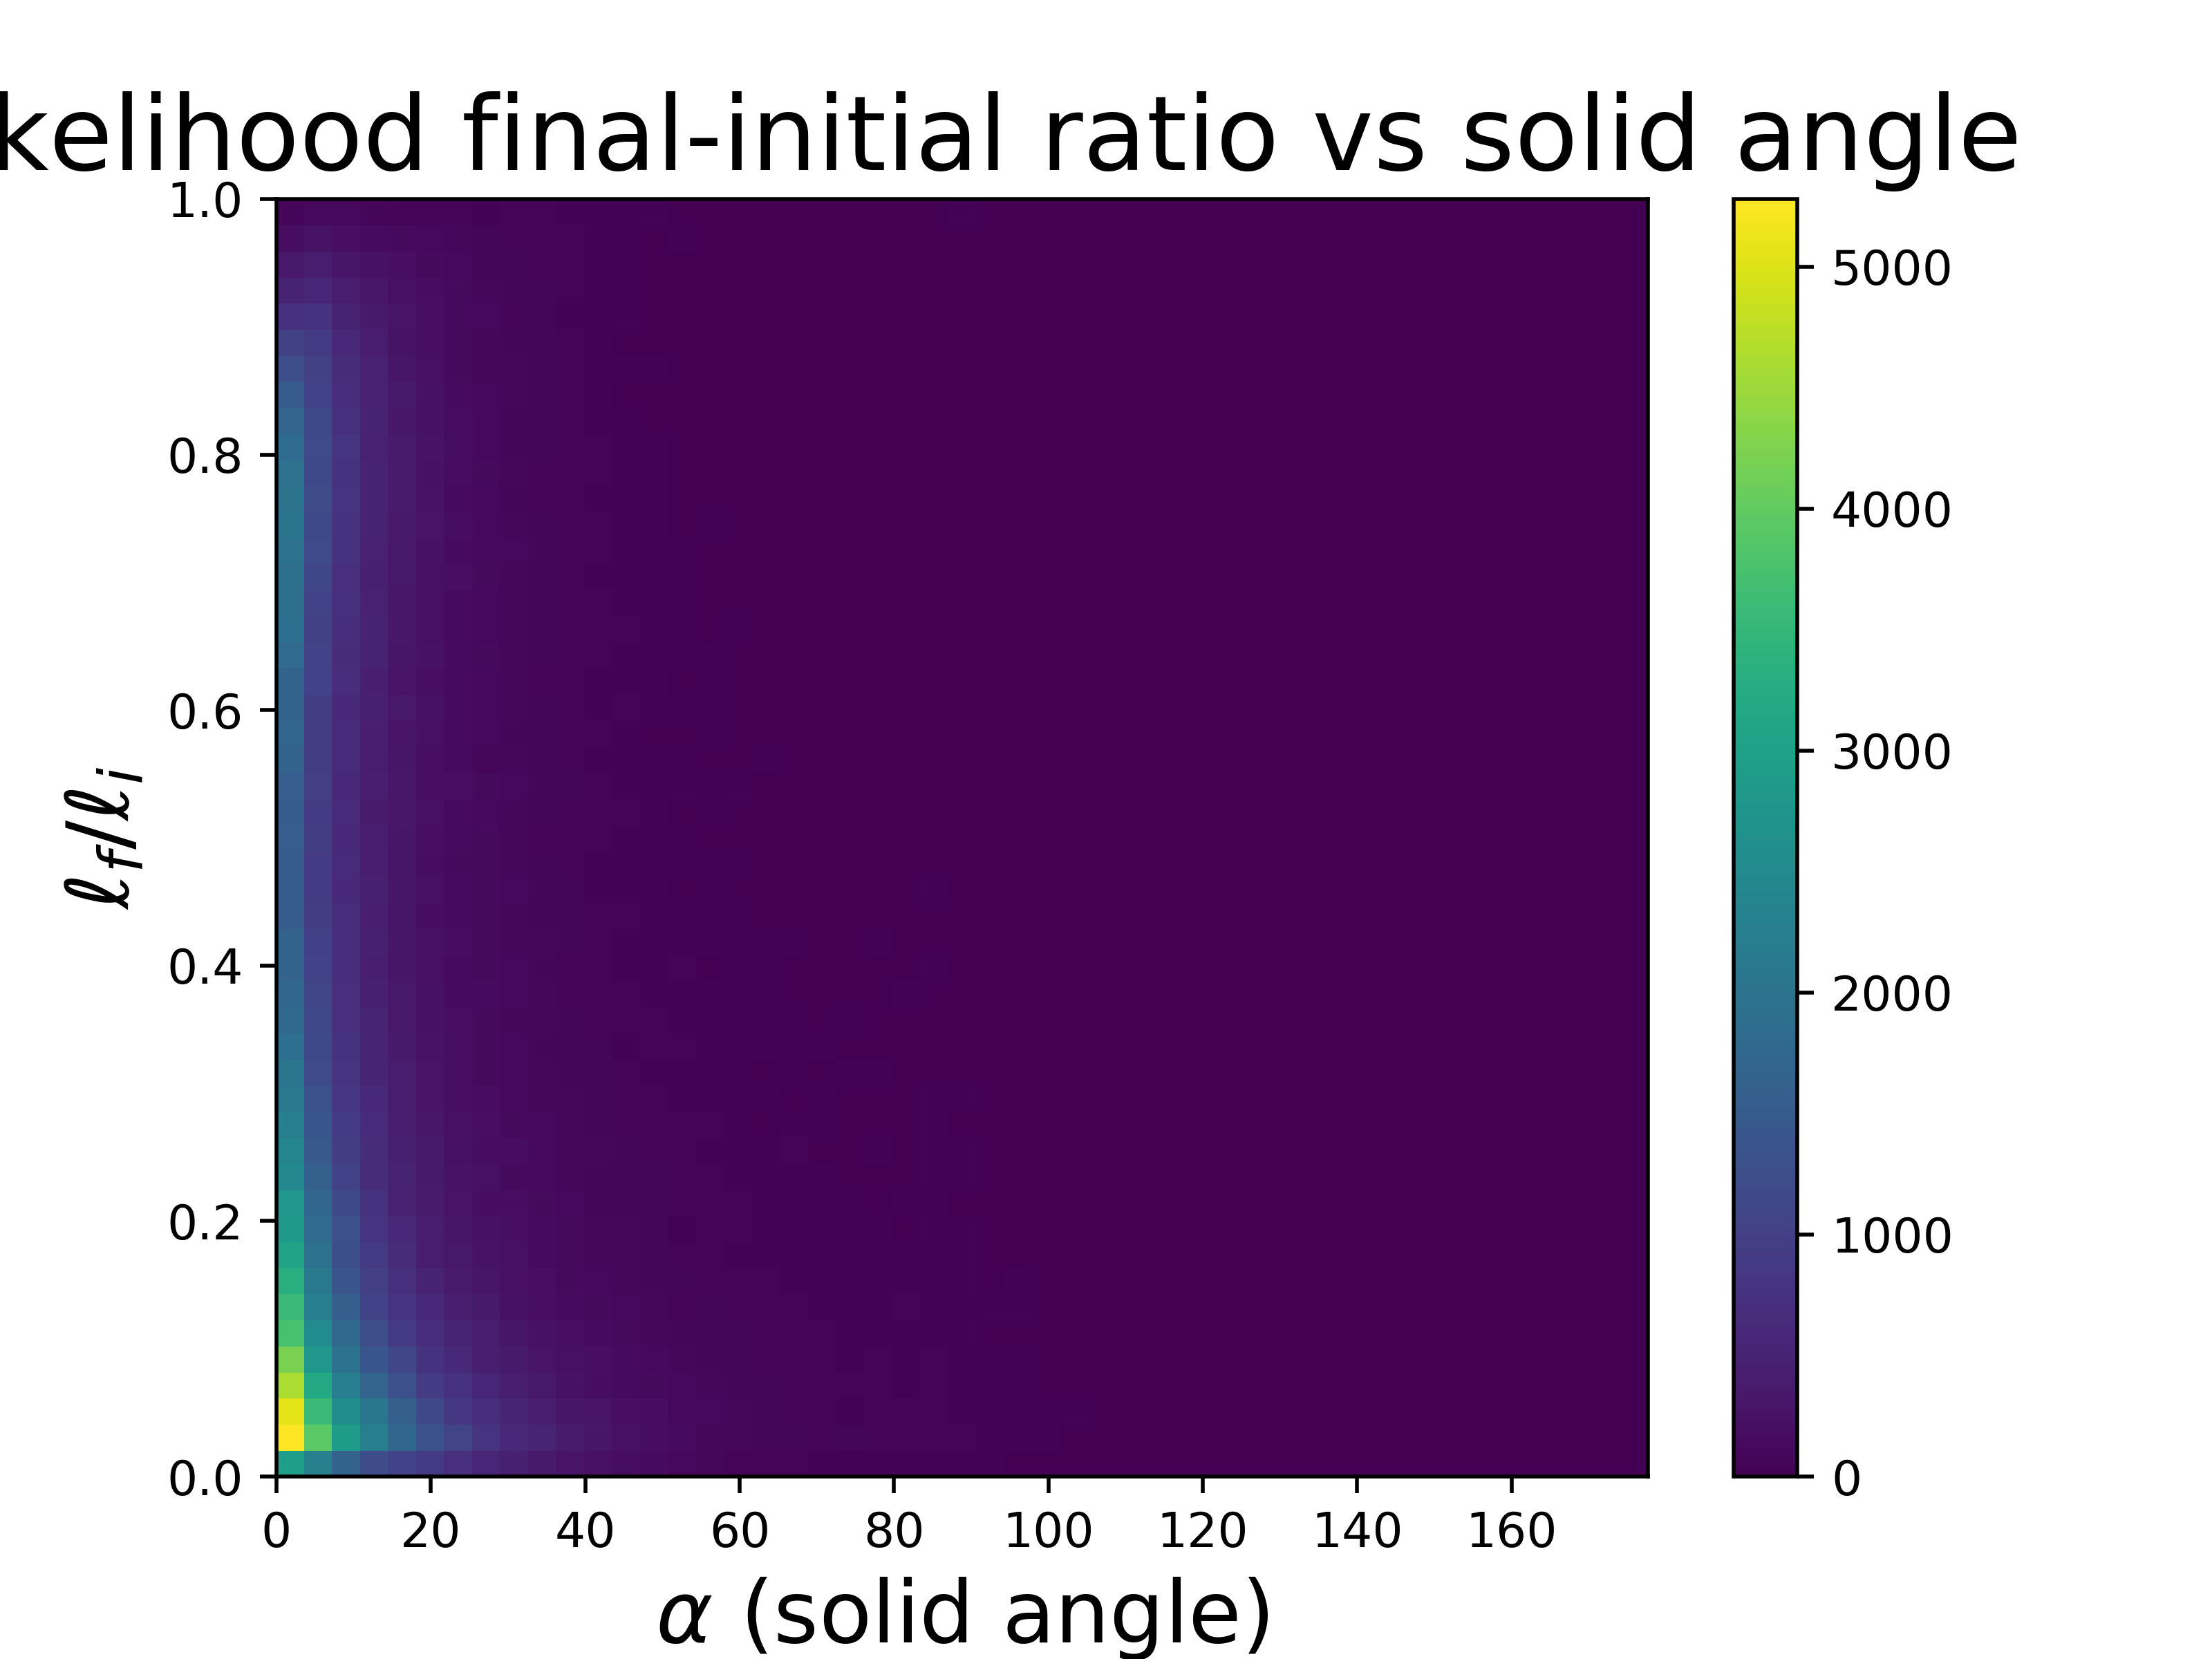
\includegraphics[width=12cm]{./Figures/reco_plots/alpha_dist_vs_llhratio_heat.png}
  \caption{We plot the likelihood ratio $\ell_{f}/\ell_{i}$ against the final reconstructed angular resolution using a heatmap. }
  \label{fig:alpha_llhratio_comp}
\end{figure}

Referring to figure \ref{fig:alpha_llhratio_comp}, we see that the events are bunching up near a small ratio of $\ell_{f}/\ell_{i}$ and small error in the solid angle $\alpha$. This could point to a correlation between the increase in the quality of the fit and the increase in the direcitonality of the reconstructed track. There could still be some hidden biases here that are being unaccounted for, such as reconstruction angles that begin close to the truth only changing in small amounts but having massive likelihood value swings. For this reason, we need to check for sure that there are no hidden biases in both $\ell_{f}$ against $\ell_{i}$ and $\alpha_{f}$ against $\alpha_{i}$.

\begin{figure}[ht]
  \begin{minipage}[b]{0.48\linewidth}
    \centering
    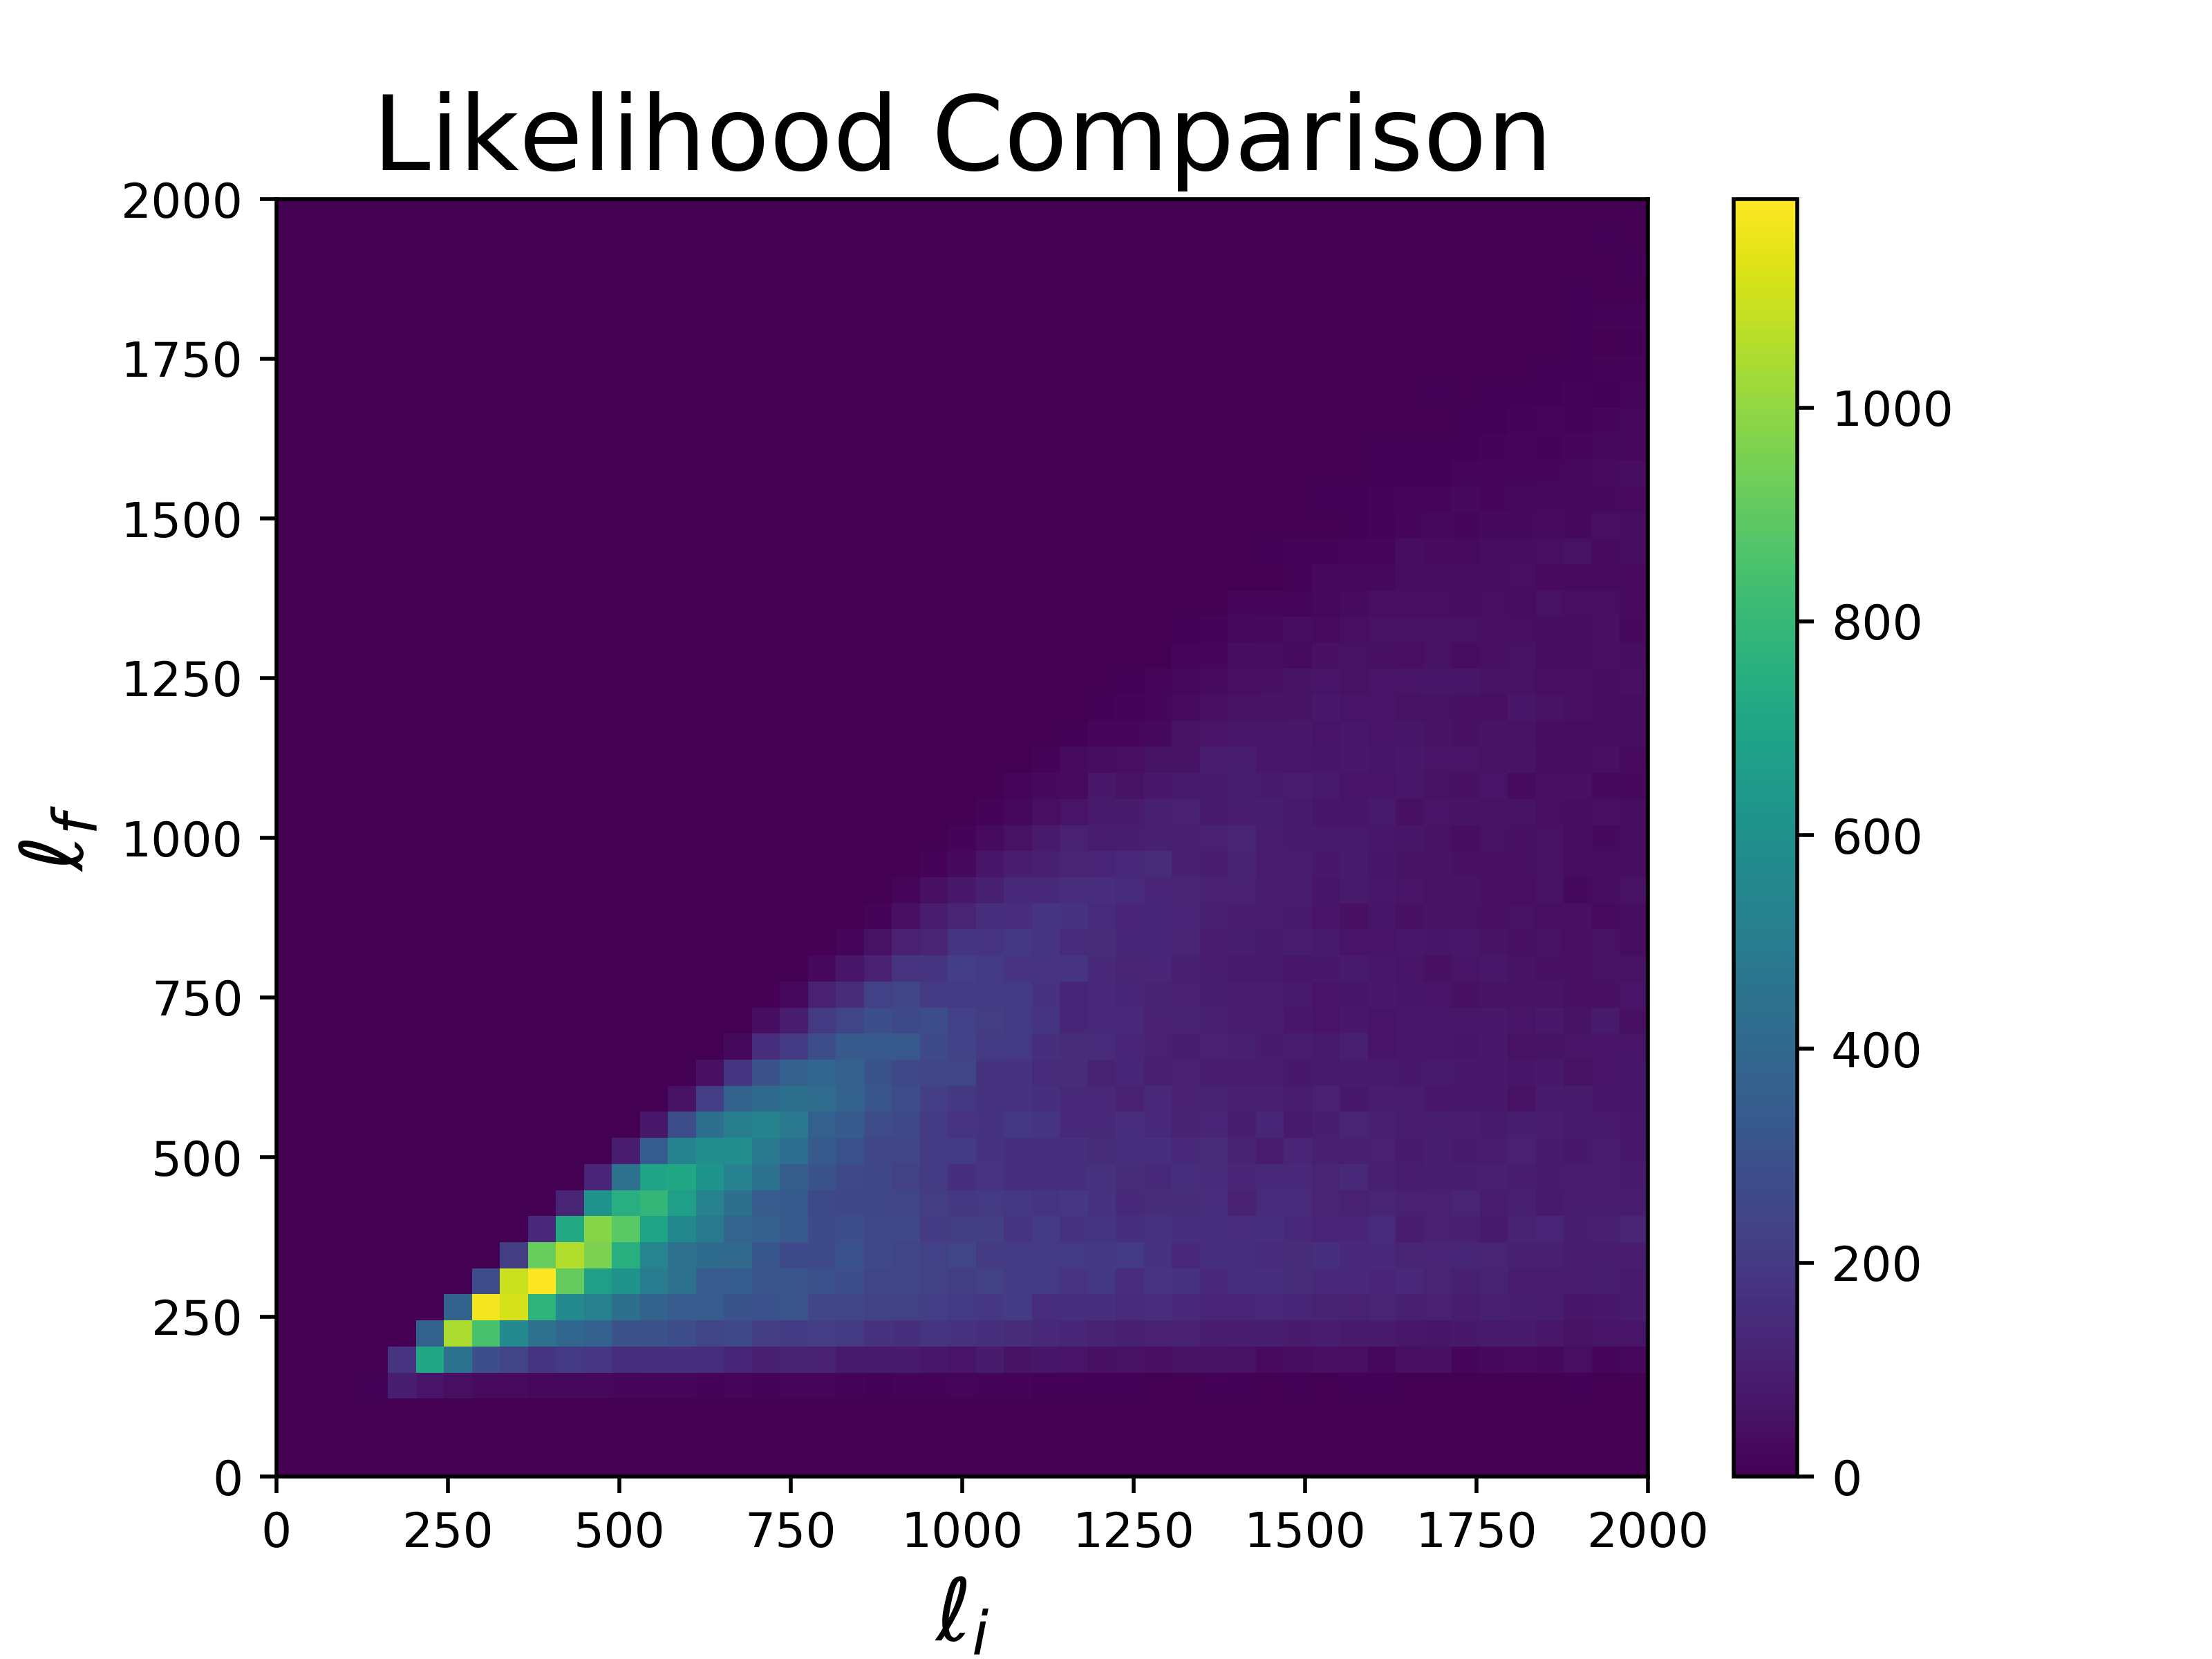
\includegraphics[width=\textwidth]{./Figures/reco_plots/llhratio_comp_heat.png}
    \caption{Correlation heatmap between the initial negative loglikelihood value and the final negative loglikelihood.}
    \label{subfig:llh_heat}
  \end{minipage}
  \hspace{0.1cm}
  \begin{minipage}[b]{0.48\linewidth}
    \centering
    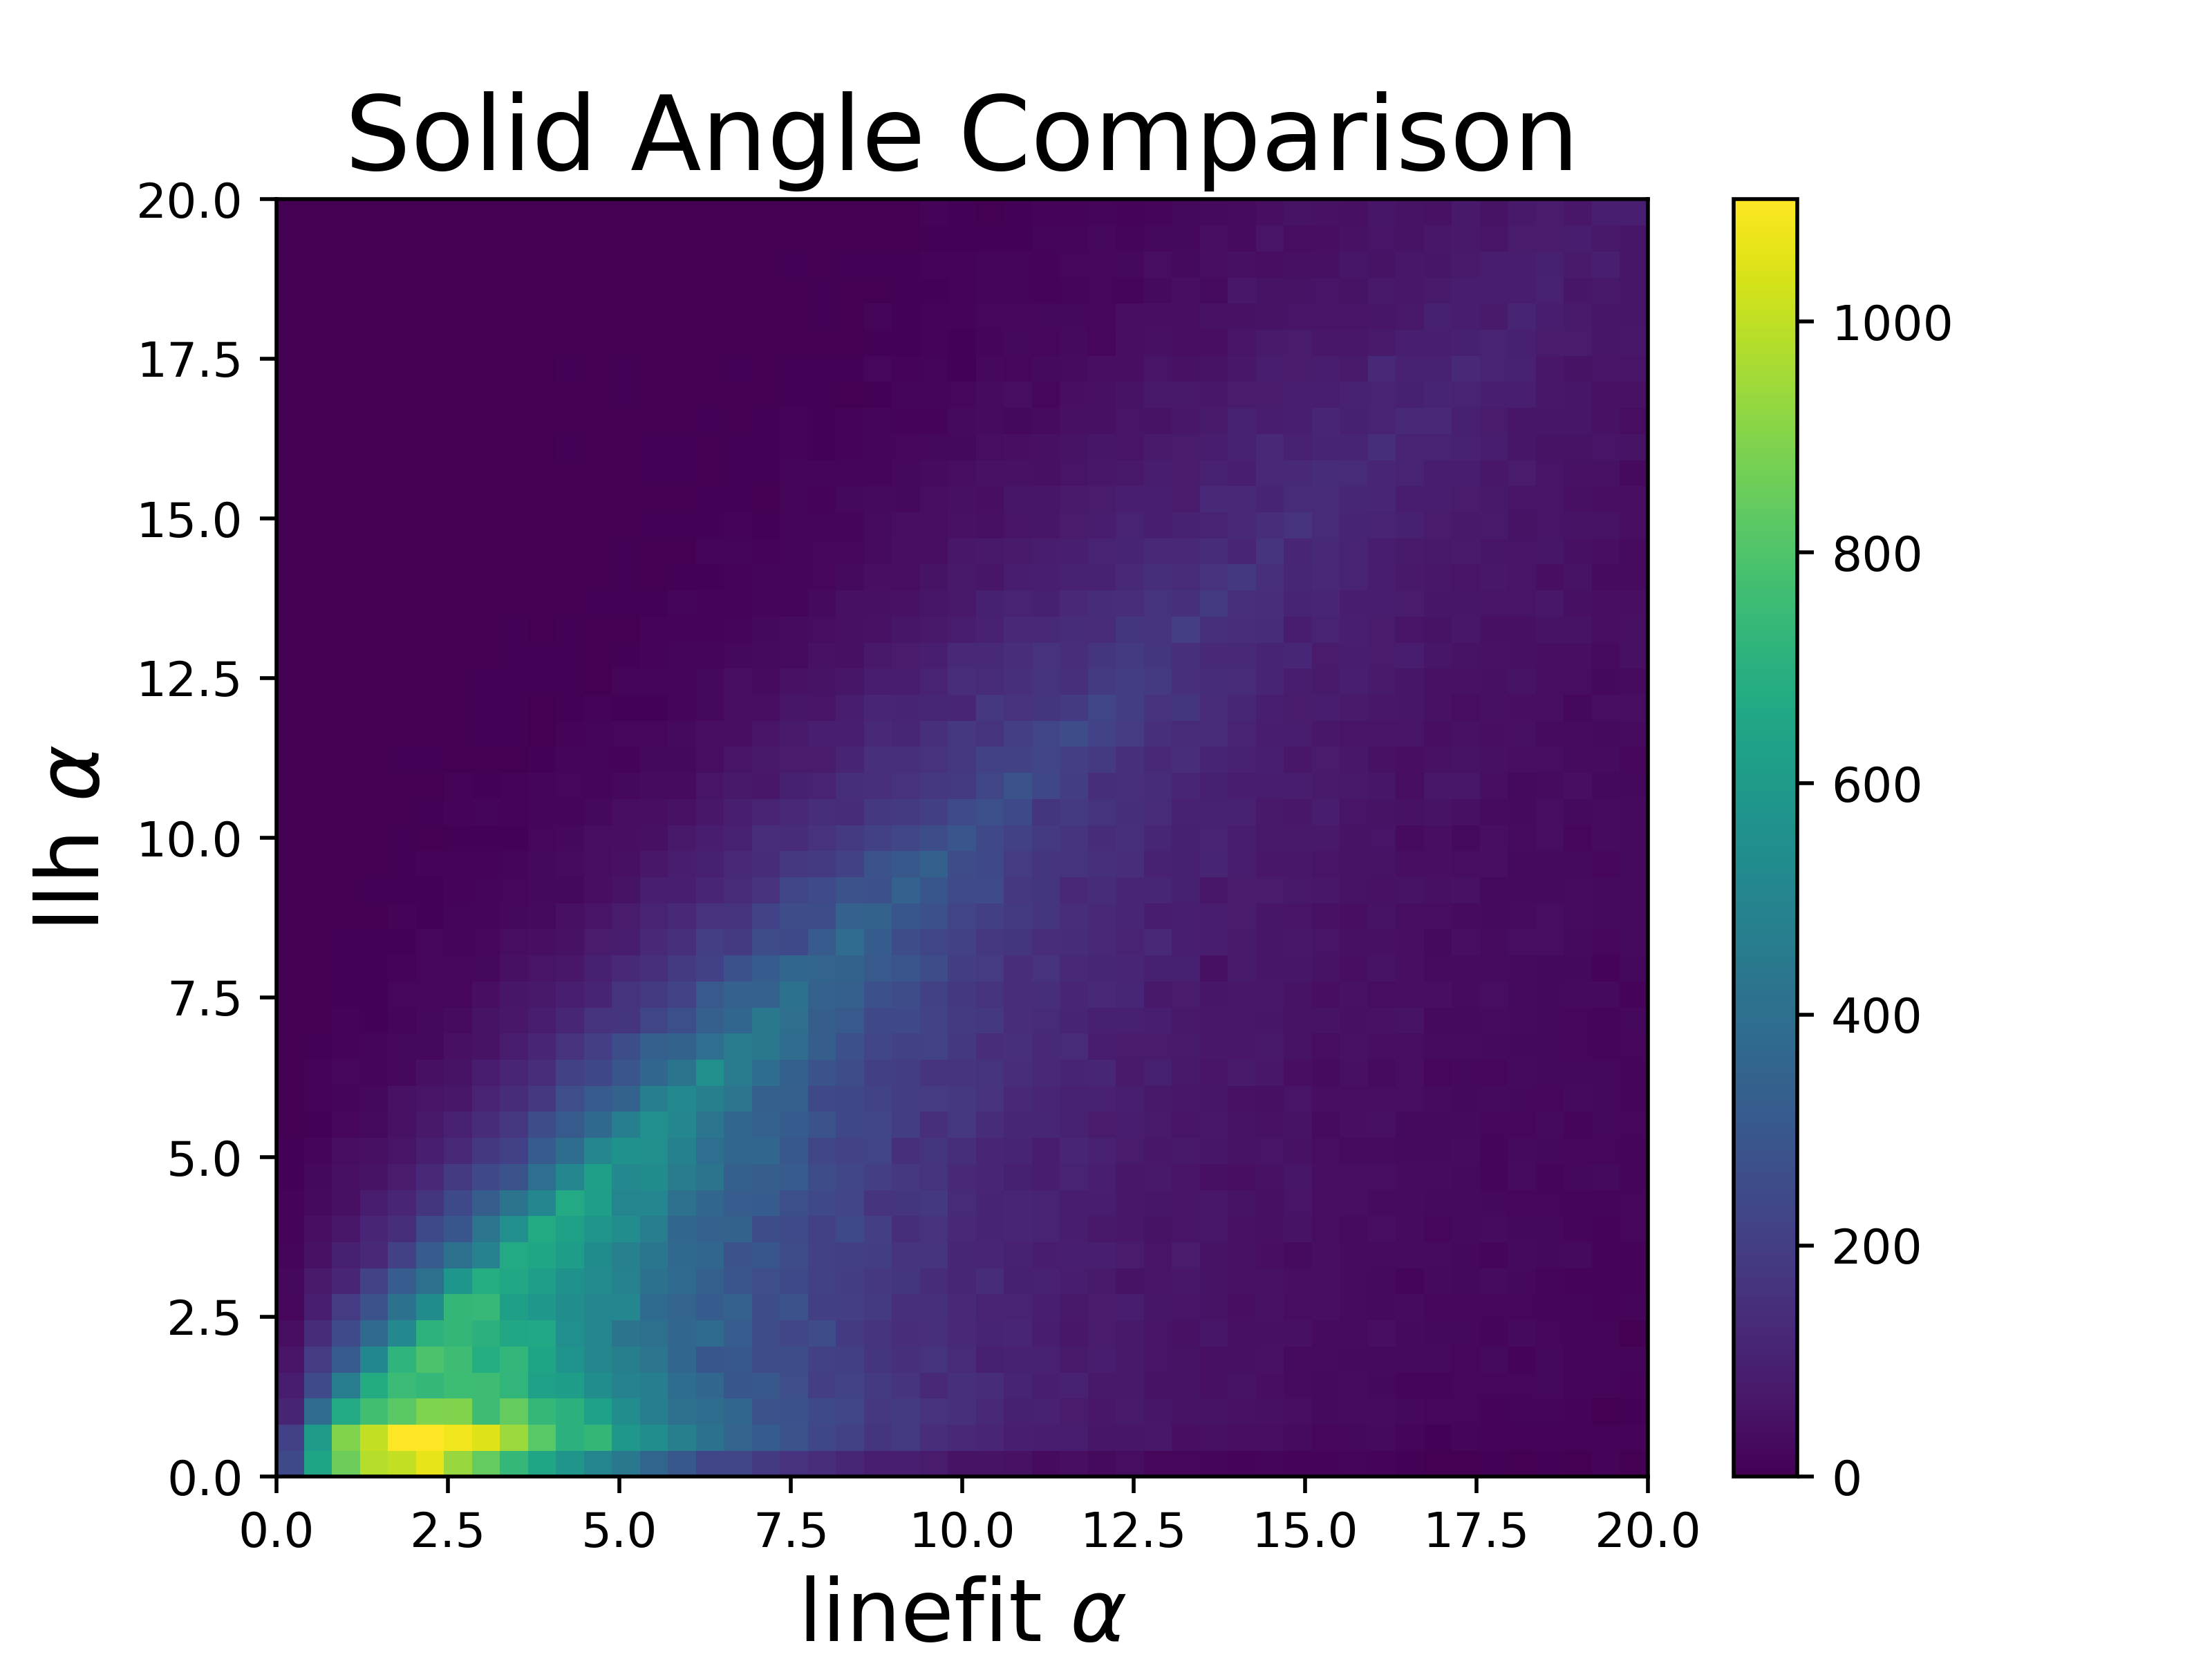
\includegraphics[width=\textwidth]{./Figures/reco_plots/alpha_dist_comp_heat.png}
    \caption{Correlation map of the final reconstructed angular resolution and the initial angular resolution.}
    \label{subfig:alpha_heat}
  \end{minipage}
\end{figure}

Looking at figures \ref{subfig:llh_heat} and \ref{subfig:alpha_heat}, we can see that the reconstruction is behaving as one would expect. For both plots, the $y=x$ diagonal line would symbolize neither improvement nor regression, and anything below would suggest improvement. In both figures majority of the points end up below this line encouraging the correlation between the reconstruction improving both the likelihood value but also the reconstructed angular direction. For figure \ref{subfig:llh_heat}, the clustering of events shows a correlation between good seed events leading to well fit final fits. The further the seed events get from being good fits, the more spread the quality of the final fit becoms. A similar result can be seen with the angular resolution correlation plot in figure \ref{subfig:alpha_heat}.

Another important parameter to consider when looking at reconstructions is the time it takes to run. This can become increasingly important as there are massive amounts of potential events a detector can observe during its runtime, and being able to reconstruct them becomes an important potential bottleneck. 

\begin{figure}[H]
  \centering
  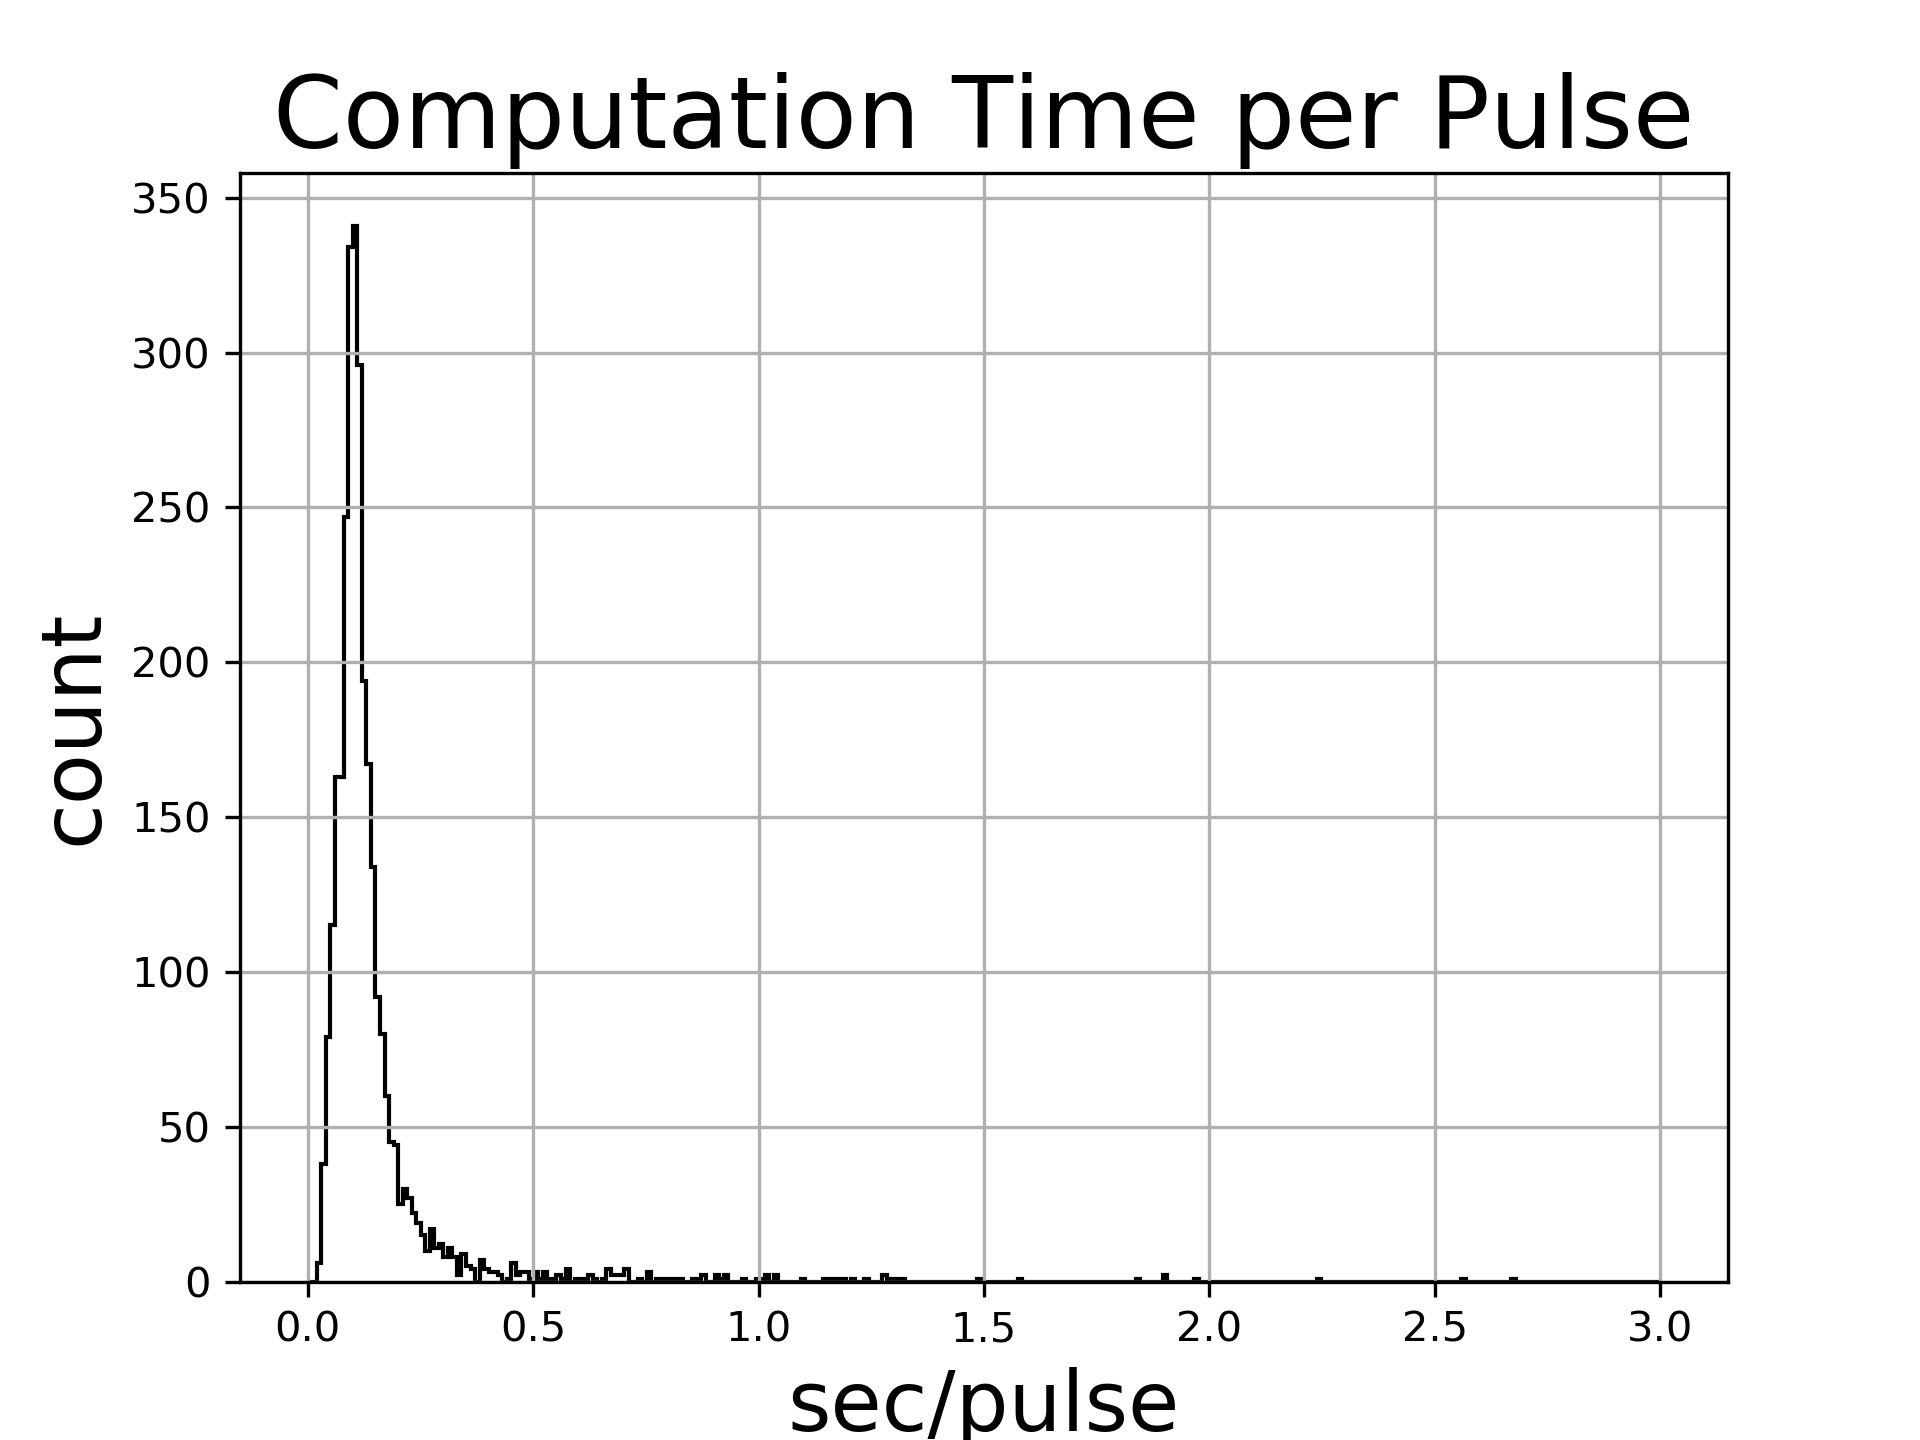
\includegraphics[width=12cm]{./Figures/reco_plots/computation_time_perpulse.png}
  \caption{Distribution of the computation time for reconstructing events normalized by the pulse count. Higher energy events will naturally need to a larger number of observed pulses and increase the computation time accordingly. }
  \label{fig:comp_time}
\end{figure}

Figure \ref{fig:comp_time} plots the computation time for the reconstruction algorithm normalized by the pulse count, where the pulse count scales with the number of photons produced, and hence the energy of the muon.


computation time

what affects the reco the most



%\chapter{Alloy}\label{ch:Alloy}

\section{The Alloy Language}

    %\gloss{Alloy} is...
    Alloy is...

\paragraph{Quantifiers}

        There are five quantifiers available in Alloy:

        \begin{center}
        \begin{singlespacing}
        \begin{tabular}{|l|l|} \hline
        % after \\: \hline or \cline{col1-col2} \cline{col3-col4} ...
        \multicolumn{1}{|c|}{Quantifier} & \multicolumn{1}{c|}{Meaning} \\ \hline
        \texttt{all x :~e | F} & universal, \texttt{F} is true for every \texttt{x} in \texttt{e} \\
        \texttt{some x :~e | F} & existential, \texttt{F} is true for some \texttt{x} in \texttt{e} \\
        \texttt{no x :~e | F} & \texttt{F} is true for no \texttt{x} in \texttt{e} \\
        \texttt{sole x :~e | F} & \texttt{F} is true for at most one \texttt{x} in \texttt{e} \\
        \texttt{one x :~e | F} & \texttt{F} is true for exactly one \texttt{x} in \texttt{e} \\ \hline
        \end{tabular}
        \end{singlespacing}
        \end{center}


\subsubsection{Signatures and Fields}

        The simple signature \verb|sig A {}| introduces \texttt{A} as a basic type with a set
        of atoms of that type.  \texttt{A} refers to the set of atoms; the type is inferred
        by Alloy and cannot be referenced explicitly.

        \begin{singlespacing}
        \begin{verbatim}
        sig A {}
        sig B {
            f : A
        }        \end{verbatim}
        \end{singlespacing}


\subsection{Example}\label{sec:firstAlloyExample}

    An excerpt from an Alloy
    specification of a singly-linked list is presented in
    Listing~\vref{list:simpleLinkedList}.

    \begin{Listing}
    \begin{singlespacing}
    {\small
    \begin{verbatim}
    sig Node {                    sig List {
        next : option Node            first : Node
    }                             }{
                                      all n : Node | n in first.*next
                                      no n : Node | n in n.^next
                                  }    \end{verbatim}
    }
    \caption{Excerpt of a simple Alloy specification for a singly-linked list}
    \label{list:simpleLinkedList}
    \end{singlespacing}
    \end{Listing}


%\chapter{Embee: User Perspective}\label{ch:Embee1}

    \begin{Listing}[H]
    \filein{Examples/List.als}
    \caption{Alloy specification of a singly-linked list using only binary relations}
    \label{list:SimpleList1}
    \end{Listing}


\subsection{Phase 1: High-Level Static Mapping}\label{sec:phase1}

    ...Phase 1 simply generates the default static
    mapping and presents it to the user, as shown in Figure~\vref{fig:defaultMap}.  We
    have modified the map file as shown in Figure~\vref{fig:fixedMap}.

    \begin{figure}[H]
    \begin{singlespacing}
    \centering
        \subfigure[Default static mapping]{
            \begin{minipage}{2.25in}\footnotesize
                {\texttt{List = List\\
                List\$first =
                List.first\\
                Node = Node\\
                Node\$next = Node.next\\
                }
                }\label{fig:defaultMap}
            \end{minipage}}
        \subfigure[Modified static mapping]{
            \begin{minipage}{2.25in}\footnotesize
                {\texttt{List = SimpleList\\
                List\$first = SimpleList.first\\
                Node = Node\\
                Node\$next = Node.next\\
                }
            }\label{fig:fixedMap}
            \end{minipage}}
    \caption[Excerpt of high-level static mapping file]{Excerpt of high-level static
    mapping file before and after modification}
    \end{singlespacing}
    \end{figure}



    Figure~\vref{fig:tree_beforeAndAfter} shows the tree
    before and after deletion, with correctly implemented code.
    Figure~\vref{fig:tree_commentedOut_mainBody} shows the tree after deletion of the
    root, when the \texttt{root = n2} statement is not executed.

    \begin{figure}[H]
    \centering
    \mbox{
        %\subfigure[Before deletion]{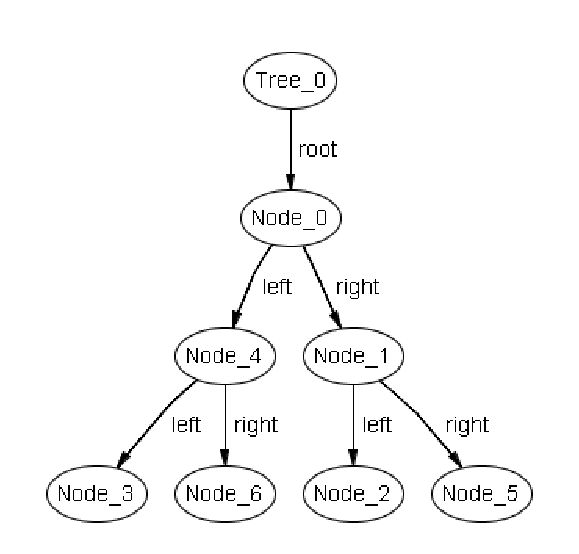
\includegraphics[scale=0.65]{Figures/correct_pre.eps}}\label{fig:tree_correct_pre}
        %\subfigure[After correct deletion]{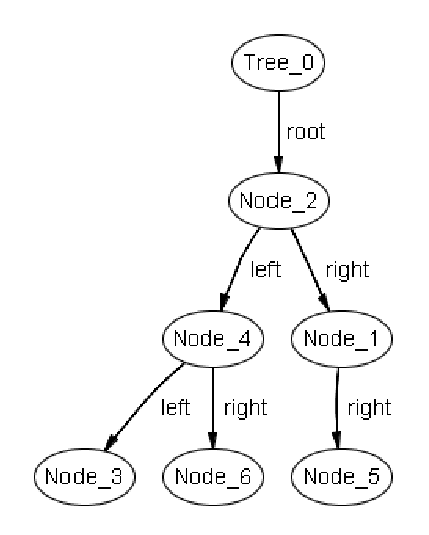
\includegraphics[scale=0.65]{Figures/correct_post.eps}}\label{fig:tree_correct_mainBody}
        \subfigure[Before deletion]{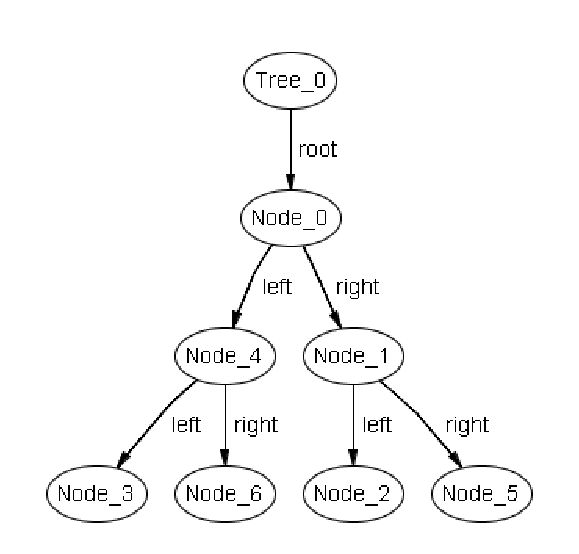
\includegraphics[scale=0.65]{Figures/correct_pre}}\label{fig:tree_correct_pre}
        \subfigure[After correct deletion]{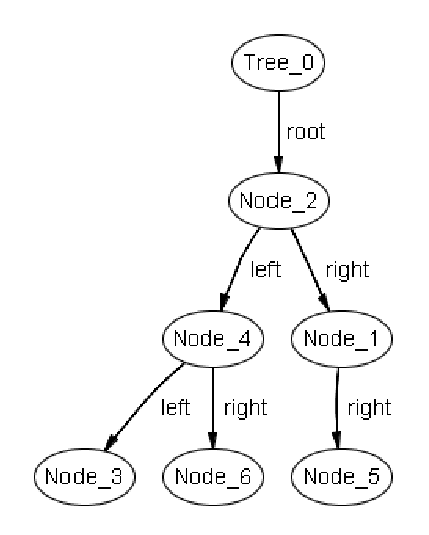
\includegraphics[scale=0.65]{Figures/correct_post}}\label{fig:tree_correct_mainBody}     
        }
    \caption[Visualization of tree]{Visualization of tree before and after correct deletion of the root node}
    \label{fig:tree_beforeAndAfter}
    \end{figure}

    \begin{singlespacing}
    \begin{figure}[H]
    \centering
    %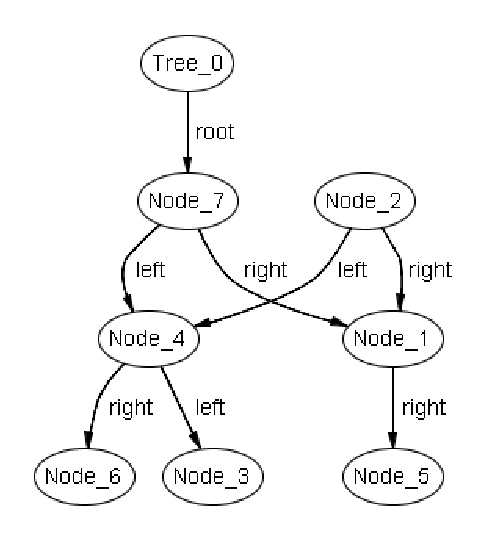
\includegraphics[scale=0.75]{Figures/commentedOutWithBetterNumber_post.eps}
    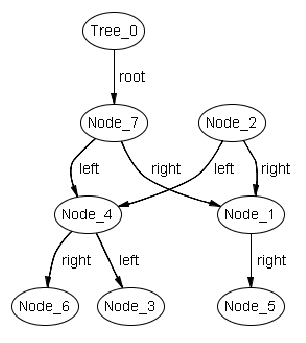
\includegraphics[scale=0.75]{Figures/commentedOutWithBetterNumber_post}
    \caption[Visualization of tree after deletion of root (error or omission)]{Visualization of tree
    after deletion of the root node, with an error of omission in the code.
    \texttt{Node\_7} represents the temporary node in the \texttt{swapNodes()} method.}
    \label{fig:tree_commentedOut_mainBody}
    \end{figure}
    \end{singlespacing}

%\chapter{Embee: Implementation and Analysis}\label{ch:Embee2}


    \begin{singlespacing}
    \begin{Listing}[h]
    \fileinsmall{Examples/connectToVM.txt} \caption[Excerpt from
    \texttt{StateDumperThreads.java}]{Excerpt from \texttt{StateDumperThreads.java},
    showing how to connect to a second virtual machine executing the target code.  In
    this example, the target class is referenced by \texttt{javaClassName}.  The JPDA
    classes can be accessed by including the \texttt{tools.jar} archive in the program's
    classpath; this archive is found in the Java installation's \texttt{lib} directory}
    \label{list:connectToVM}
    \end{Listing}
    \end{singlespacing}


    \begin{figure}[h]
    \begin{singlespacing}
    \centering
        \subfigure[Specification of binary \texttt{next} relation]{
            \begin{minipage}{100pt}
                \filein{Examples/smallA.txt}
            \label{fig:smallBinary}
            \end{minipage}}
        \hspace{0.25in}
        \subfigure[Implementation of binary relation in (a)]{
            \begin{minipage}{100pt}
                \filein{Examples/smallB.txt}
            \label{fig:smallBinaryCode}
            \end{minipage}}
        \hspace{0.25in}
        \subfigure[Specification of ternary \texttt{next} relation]{
            \begin{minipage}{100pt}
                \filein{Examples/smallC.txt}
            \label{fig:smallTernary}
            \end{minipage}}
    \caption[Sample specification and implementation]{Sample specification and
    implementation of a binary relation; sample specification of a ternary relation}
    \end{singlespacing}
    \end{figure}

\section{Complexity and Performance}\label{sec:EmbeeComplexity}

\subsection{Definition of Terms}\label{sec:termDefn}

    The following terms...:

    \begin{Ventry}{\boldmath $\operatorname{arity}(r_i)$ \unboldmath}

        \boldmath \item[$scope$] \unboldmath
        The maximum number of objects...

        \boldmath \item[$R$] \unboldmath
        The number of relations...

        \boldmath \item[$r_i$] \unboldmath
        The $i^\text{th}$ relation in the specification, $1 \le i \le R$.

        \boldmath \item[$\operatorname{arity}(r_i)$] \unboldmath
        The arity of relation $r_i$...

        \boldmath \item[$N$] \unboldmath The total number...

        Given the calculated arities of a particular specification's relations, and the scope at
        a specific breakpoint, Equation~\ref{equation:N} can be used to determine $N$.
        \begin{equation}\label{equation:N}
        N = S \times scope + \sum_{i=1}^R scope ^ {arity(r_i)}
        \end{equation}

    \end{Ventry}



    The combined complexity of all four steps is
    \begin{equation*}
        O(N) + O(nN) + O(N^2) + O(F)
    \end{equation*}
    Again, these steps are completed once for every breakpoint in the target program's
    execution; therefore, the overall upper bound becomes
    \begin{equation*}
    \begin{split}
        & b \times O(N) + b \times O(nN) + b \times O(N^2) + b \times  O(F) \\
                   = ~ & O(bN + bnN + bN^2 + bF)
    \end{split}
    \end{equation*}


    The vector [$x_0$  $x_1$] represents the two possible atoms of type
    \texttt{X}.  With our naming scheme, $x_0$ represents \texttt{X\_0} and $x_1$
    represents \texttt{X\_1}.
    The binary relation itself is represented by a two-dimensional bit matrix where a 1 in
    position [$i$,$j$] means that there is a mapping between the $i^{th}$ atom of \texttt{X}
    and the $j^{th}$ atom of \texttt{Y}:

    \begin{gather*}
    \begin{bmatrix}
      r_{00} & r_{01} \\
      r_{10} & r_{11} \\
    \end{bmatrix} \quad
    \begin{bmatrix}
      \texttt{X\_0->Y\_0} & \texttt{X\_0->Y\_1} \\
      \texttt{X\_1->Y\_0} & \texttt{X\_1->Y\_1} \\
    \end{bmatrix}
    \end{gather*}
    \medskip

    Now, consider a fact stating that relation \texttt{r} is total, i.e.,

    \begin{center}
    \texttt{all x :~X | some y :~Y | x.r = y}
    \end{center}

    The CNF formula for our example fact, in scope~2, is
    \begin{equation*}
    \begin{split}
    & \neg(((x_0 \wedge r_{00}) \vee (x_1 \wedge r_{10})) \wedge \neg((x_0 \wedge r_{01})
    \vee (x_1 \wedge r_{11}))) \wedge \\ &\neg(\neg((x_0 \wedge r_{00}) \vee (x_1 \wedge
    r_{10})) \wedge ((x_0 \wedge r_{01}) \vee (x_1 \wedge r_{11})))
    \end{split}
    \end{equation*}
    \medskip

    Table~\vref{fig:fullRunTimesAllPhases} contains...

    \begin{singlespacing}
    \begin{center}
    \begin{threeparttable}
    \caption{Running times for each phase and total running time of Embee}
    \label{fig:fullRunTimesAllPhases}\begin{small}
        % Table generated by Excel2LaTeX from sheet 'Embee'
        \begin{tabular}{|l|c|c|c|c|c|c|c|} \hline

        \multicolumn{3}{|c|}{Test Case} & \multicolumn{ 5}{c|}{Running Time (m:ss)} \\ \hline

        \multicolumn{1}{|c|}{Object} & & Number of & & & \multicolumn{2}{c|}{ Phase 3} &  \\  \cline{6-7}

        \multicolumn{1}{|c|}{Model} & \raisebox{1.5ex}[0pt]{Scope} & Breakpoints &  \raisebox{1.5ex}[0pt]{Phase 1} & \raisebox{1.5ex}[0pt]{Phase 2} &   First 16 &   Last 4 &  \raisebox{1.5ex}[0pt]{Total} \\

        \hline
            List  &  20 &  20           &  0:07 &  0:32 &  0:12 &  06:39 & 07:30 \\
        \hline
            Graph &  20 &  19\tnote{a}  &  0:07 &  1:27 &  0:35 &  44:10 & 46:19 \\
        \hline
            Tree  &  20 &  20 &  0:04   &  1:20 &  0:21 &  06:04 &  07:49 \\
        \hline
        \end{tabular}
    \begin{tablenotes}
    \item[a] Breakpoints occur after the addition of each edge, i.e., the first
    breakpoint does not occur until the second node is added.
    \end{tablenotes}
        \end{small}
    \end{threeparttable}
    \end{center}
    \end{singlespacing}


    ...upper bound on Embee's performance:

    \begin{numcases}{\text{upper bound is}}
        O(bN^2) & if $scope \leq 16$ \notag \\
        O(bF)   & if $scope > 16$ \notag
    \end{numcases}



\chapter{Summary and Conclusions}\label{ch:Conclusion}

\section{Summary}

\section{Future Work}

\section{Conclusion}


%*************************************************************************************************************
% BIBLIOGRAPHY
%*************************************************************************************************************
% This GATHER command is useful for when you want to use WinEdt's Gather functionality, i.e., type
% \cite{} and a popup box appears with all of your citations to choose from.  Leave the % on the next line.
%GATHER{thesis.bib}

% Put in \nocite{*} so all entries in the bibliography are included
%\nocite{*}

\bibliographystyle{plain}
\bibliography{thesis}

%*************************************************************************************************************
% APPENDICES
%*************************************************************************************************************
\updatechaptername
%\appendixpage
\appendix

%\chapter{Alloy Analyzer}\label{App:AnalyzerCode}

\section{Documentation}

\paragraph*{\large Package: \texttt{alloy.api}}

    %%%%%%%%%%%%%%%%%%%%%%%%%%%%%%%%%%%%%%%%%%%%%%%%%%%%%%%%%%%%
    % AlloyRunner
    %%%%%%%%%%%%%%%%%%%%%%%%%%%%%%%%%%%%%%%%%%%%%%%%%%%%%%%%%%%%
    \begin{singlespacing}
    \begin{center}
    \begin{tabularx}{\linewidth}{|l|X|} \hline
    \multicolumn{2}{|p{420pt}|}{\texttt{\large AlloyRunner}} \\ \hline \hline

    \multicolumn{2}{|p{420pt}|}{\small This class provides...} \\
    \multicolumn{2}{|p{420pt}|}{} \\
    \multicolumn{2}{|p{420pt}|}{\small To do an analysis...}\\ \hline \hline

    {\small \texttt{analyzeCommand}} & {\small Run the actual...} \\ \hline

    {\small \texttt{prepareSpec}} & {\small Parse...} \\ \hline

    {\small \texttt{translateCommand}} & {\small Translate...} \\
    \hline

    \end{tabularx}
    \end{center}
    \end{singlespacing}

%\chapter{Additional Analysis}\label{App:Analysis}

\section{Calculation of Arity}\label{AppSec:arity}


    Examples of arity calculations are shown in Table~\vref{table:arity}.  These calculations
    can be performed using either the equations listed in
    Figure~\vref{fig:arityEquations}...

   \begin{singlespacing}
    \begin{figure}[ht]
    \begin{boxedminipage}[h]{433pt}
        \begin{minipage}{400pt}

        Given:
            \begin{center}
            \begin{minipage}{350pt}
            $v$ is a variable of type \texttt{<var>}, i.e., an \texttt{id} (identifier)\\
            $m$ is a multiplicity expression of type \texttt{<multexpr> }\\
            $r$ is a relation of type \texttt{<relation>}, i.e., $r = v : m$ \\
            $e_1$, $e_2$, ... are expressions of type \texttt{<expr> }in $m$\\
            $x$ is an optional set multiplicity modifier of type \texttt{<setmult>}\\
            $y$, $z$ are optional relation multiplicity modifiers of type \texttt{<mult>}
            \end{minipage}
            \end{center}
        The arity equations are:
        \end{minipage}
        \begin{equation}
        \operatorname{arity}(r) = 1 + \operatorname{arity}(m) \text{,~~where $r$ is of the form $v : m$}
        \label{equation:arity1}
        \end{equation}
        \begin{subequations}
        \begin{numcases}{arity(m)=}
            1 & if $m$ is of the form $x~v$ \label{equation:arity2a} \\
            arity(e_1) + arity(e_2) & if $m$ is of the form $e_1 ~y$ \texttt{->} $z~ e_2$ \label{equation:arity2b}
        \end{numcases}
        \end{subequations}
        \begin{subequations}
        \begin{numcases}{arity(e)=}
            1 & if $e$ is of the form \texttt{id} \label{equation:arity3a} \\
            arity(e_1) & if $e$ is of the form $(e_1)$ \label{equation:arity3b} \\
            arity(e_1) + arity(e_2) & if $e$ is of the form $e_1$ \texttt{->} $e_2$ \label{equation:arity3c}
        \end{numcases}
        \end{subequations}
        \label{equation:arityEquations}
    \end{boxedminipage}
    \caption{Equations to compute arity of relations} \label{fig:arityEquations}
    \end{figure}
    \end{singlespacing}

        \begin{singlespacing}
        \begin{table}[H]
        \begin{center}
        \caption{Example arity calculations}\label{table:arity}
        \bigskip
        \begin{tabular}{|l|c|c|}\hline
        \multicolumn{1}{|c|}{relation $r_i$} & \multicolumn{1}{c|}{$arity(r_i)$} & \multicolumn{1}{c|}{arity equations used} \\ \hline
        \verb|f : A |                    & 2 & \eqref{equation:arity1}, \eqref{equation:arity2a} \\ \hline
        \verb|f : option A|              & 2 & \eqref{equation:arity1}, \eqref{equation:arity2a} \\ \hline
        \verb|f : A -> A|                & 3 & \eqref{equation:arity1}, \eqref{equation:arity2b}, \eqref{equation:arity3a} \\ \hline
        \verb|f : A -> ? B|              & 3 & \eqref{equation:arity1}, \eqref{equation:arity2b}, \eqref{equation:arity3a} \\ \hline
        \verb|f : A -> B -> C|           & 4 & \eqref{equation:arity1}, \eqref{equation:arity2b}, \eqref{equation:arity3c}, \eqref{equation:arity3a} \\ \hline
        \verb|f : A -> B ? -> ! C|       & 4 & \eqref{equation:arity1}, \eqref{equation:arity2b}, \eqref{equation:arity3a}, \eqref{equation:arity3c} \\ \hline
        \verb|f : A -> B -> C -> D|      & 5 & \eqref{equation:arity1}, \eqref{equation:arity2b}, \eqref{equation:arity3c}, \eqref{equation:arity3a} \\ \hline
        \end{tabular}
        \end{center}
        \end{table}
        \end{singlespacing}

\section{Comparison of $N$}\label{AppSec:CompareN}



\subsection{Reasoning about $N$ in terms of $n$}\label{AppSec:Nandn}

    It is possible to determine an upper bound on the size of $N$, relative to the size
    of $n$.  To do this, we re-examine Equation~\ref{equation:N}.

    From Equation~\ref{equation:N}, we have:
    \begin{equation*}
        N = S \times scope + \sum_{i=1}^R scope ^ {arity(r_i)}
    \end{equation*}

    In the worst-case, the scope is equal to the total number of objects that exist at a
    particular breakpoint, i.e., $scope = n$.
    \begin{equation*}
        N = S n + \sum_{i=1}^R n ^ {arity(r_i)}
    \end{equation*}

    We can expand the summation to
    \begin{equation*}
        N = S n + n^{arity(r_1)} + n^{arity(r_2)} + ... + n^{arity(r_R)}
    \end{equation*}

    Because...
    \begin{equation*}
        O(N) = O(S n) + O(n^{arity(r_1)}) + O(n^{arity(r_2)}) + ... +
        O(n^{arity(r_R)})
    \end{equation*}

    We assume that all $R$ relations in the specification have the same arity, and that this
    arity is represented by a value $x \geq 2$.  Therefore...
    \begin{align}
        O(N) & = O(S n) + R \times O(n^x) \notag \\
             & = O(S n) + O(R n^x)
        \label{equation:NwithSR}
    \end{align}

    Equation~\ref{equation:NwithSR} demonstrates...

    Because both $S$ and $R$ are finite numbers, it is possible to further reduce
    Equation~\ref{equation:NwithSR} to
    \begin{align}
        O(N) & = O(n) + O(n^x) \notag \\
             & = O(n^x)
        \label{equation:NwithoutSR}
    \end{align}

    Therefore...





\clearpage
\section{Estimation of $F$}\label{AppSec:F}

    For example, Table~\vref{table:numOperators} contains the values of $F$...

    \begin{singlespacing}
    \begin{table}[H]
    \caption[Estimate of Boolean formula size]{Estimate of Boolean formula size,
    determined by number of Boolean operators (``and", ``or", ``not")}
    \label{table:numOperators}
        \begin{center}

        \bigskip

        % Table generated by Excel2LaTeX from sheet 'formula (extract)'
        \begin{tabular}{|c|r|r|r|r|}
        \hline
            \multicolumn{ 5}{|c|}{\textbf{Example 1 - List}} \\
        \hline
            $scope$ & \multicolumn{1}{c|}{$N$} & \multicolumn{1}{c|}{0 Facts} & \multicolumn{1}{c|}{1 Fact} & \multicolumn{1}{c|}{2 Facts} \\
        \hline
                1 &  4 &    23  &     34  &     43  \\
                2 & 12 &   197  &    657  &    729  \\
                3 & 24 &   671  & 13,799  & 15,200  \\
                4 & 40 & 1,731  & 91,435  & 96,771  \\
        \hline
        \end{tabular}

        \bigskip

        % Table generated by Excel2LaTeX from sheet 'formula (extract)'
        \begin{tabular}{|c|r|r|r|r|r|}
        \hline
            \multicolumn{ 6}{|c|}{\textbf{Example 2 - Graph}} \\
        \hline
            $scope$ & \multicolumn{1}{c|}{$N$} & \multicolumn{1}{c|}{Facts} & \multicolumn{1}{c|}{1 Fact} & \multicolumn{1}{c|}{2 Facts} & \multicolumn{1}{c|}{3 Facts} \\
        \hline
                1 & ---&   ---  &     ---  &       ---  &       ---  \\
                2 & 16 &   185  &   1,005  &     1,783  &     2,181  \\
                3 & 42 &   674  &  66,722  &   118,250  &   142,328  \\
                4 & 88 & 1,787  & 635,811  & 1,153,063  & 1,319,611  \\
        \hline
        \end{tabular}

        \bigskip

        % Table generated by Excel2LaTeX from sheet 'formula (extract)'
        \begin{tabular}{|c|r|r|r|r|r|r|}
        \hline
            \multicolumn{ 7}{|c|}{\textbf{Example 3 - Tree}} \\
        \hline
            $scope$ & \multicolumn{1}{c|}{$N$} & \multicolumn{1}{c|}{0 Facts} & \multicolumn{1}{c|}{1 Fact} & \multicolumn{1}{c|}{2 Facts} & \multicolumn{1}{c|}{3 Facts} & \multicolumn{1}{c|}{4 Facts} \\
        \hline
                1 &  7 &    39  &      78  &      93  &     103  &     104  \\
                2 & 22 &   367  &   1,601  &   2,487  &   2,629  &   2,715  \\
                3 & 45 & 1,283  &  38,528  &  73,472  &  76,196  &  76,568  \\
                4 & 76 & 3,359  & 234,595  & 456,459  & 466,979  & 468,087  \\
        \hline
        \end{tabular}
        \end{center}
    \end{table}
    \end{singlespacing}


\clearpage
\subsection{Test Series}

    Table~\vref{table:tests} summarizes...

    \begin{singlespacing}
    \begin{table}[H]
    \begin{center}
    \caption{Test series for evaluating the running time of conformance checking}
    \begin{tabular}{|c|c|c|c|c|c|c|c|c|} \hline
      % after \\: \hline or \cline{col1-col2} \cline{col3-col4} ...
      Series &  &  &  &  & Number &  &  & Number \\
      Name &
      \raisebox{1.5ex}[0cm][0cm]{Example} &
      \raisebox{1.5ex}[0cm][0cm]{$S$} &
      \raisebox{1.5ex}[0cm][0cm]{$R$} &
      \raisebox{1.5ex}[0cm][0cm]{$\operatorname{arity}(r_i)$} &
      of Facts &
      \raisebox{1.5ex}[0cm][0cm]{$scope=n$} &
      \raisebox{1.5ex}[0cm][0cm]{$N$} &
      of Tests \\ \hline

      E1F0 & 1            & 2 & 2 & 2, 2        & 0 & 1,2,...,40 & 4 - 3,280   & 40 \\ \cline{1-1} \cline{6-9}
      E1F1 & \emph{List}  &   &   &             & 1 & 1,2,...,32 & 4 - 1,984   & 32 \\ \cline{1-1} \cline{6-9}
      E1F2 &              &   &   &             & 2 & 1,2,...,31 & 4 - 1,984   & 31 \\ \hline
      E2F0 & 2            & 2 & 2 & 2, 3        & 0 & 2,3,...,40 & 16 - 65,680 & 39 \\ \cline{1-1} \cline{6-9}
      E2F1 & \emph{Graph} &   &   &             & 1 & 2,3,...,40 & 16 - 33,856 & 39 \\ \cline{1-1}\cline{6-9}
      E2F2 &              &   &   &             & 2 & 2,3,...,34 & 16 - 33,856 & 33 \\ \cline{1-1}\cline{6-9}
      E2F3 &              &   &   &             & 3 & 2,3,...,24 & 16 - 14,448 & 23 \\ \hline
      E3F0 & 2            & 3 & 4 & 2, 2, 2, 2  & 0 & 1,2,...,40 & 7 - 6,520   & 40 \\ \cline{1-1} \cline{6-9}
      E3F1 & \emph{Tree}  &   &   &             & 1 & 1,2,...,40 & 7 - 6,520   & 40 \\ \cline{1-1}\cline{6-9}
      E3F2 &              &   &   &             & 2 & 1,2,...,32 & 7 - 4,192   & 32 \\ \cline{1-1}\cline{6-9}
      E3F3 &              &   &   &             & 3 & 1,2,...,32 & 7 - 4,192   & 32 \\ \cline{1-1}\cline{6-9}
      E3F4 &              &   &   &             & 4 & 1,2,...,32 & 7 - 4,192   & 32 \\ \hline
      \multicolumn{8}{|r|}{Total Number of Tests (Conformance Checks)} & 412 \\ \hline
    \end{tabular}
    \label{table:tests}
    \end{center}
    \end{table}
    \end{singlespacing}

%\addappheadtotoc

%*************************************************************************************************************
% GLOSSARY
% Using a glossary is more than beginners need to know; leaving the packages, etc. here for now.
%*************************************************************************************************************
%\usepackage[nonumberlist]{glossaries}
%\usepackage[refpages]{gloss}  % for my glossary
                              % refpages shows the first page where the term occurs
%-------------------------------------------------------------------------------------------------------------
% Tell Latex to make a glossary
%*************************************************************************************************************
%\makeglossaries  % tell latex to make the glossary
%\glossarystyle{list}

%*************************************************************************************************************
% INDEX
%*************************************************************************************************************
% Here's where the index would be printed, if you created one.  Remove the % on the next line.
%\printindex


%*************************************************************************************************************
\end{document}
